\documentclass[../../Matt_Gebert_Honours_Thesis.tex]{subfiles}

\begin{document}
	To create graphene devices where we can measure the electronic properties referenced in \cref{sec:fet,sec:electronic_properties}, a variety of steps need to be taken in order to probe electronic flow.
	
	\begin{figure}[H]
	\centering
	\begin{subfigure}{0.2\textwidth}
		\centering
		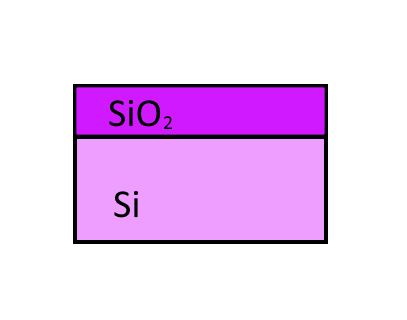
\includegraphics[width=\textwidth]{chap2/lithography/01SiliconOxide}
		\caption{Surface preparation of \silicondioxide}
	\end{subfigure}
	\hspace{0.04\textwidth}
	\begin{subfigure}{0.2\textwidth}
		\centering
		\includegraphics[width=\textwidth]{chap2/lithography/02graphene}
		\caption{Exfoliation of graphene on \silicondioxide}
	\end{subfigure}
	\hspace{0.04\textwidth}
	\begin{subfigure}{0.2\textwidth}
		\centering
		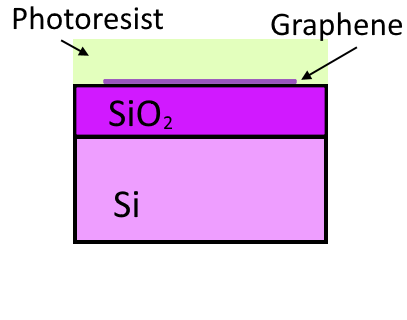
\includegraphics[width=\textwidth]{chap2/lithography/03Photoresist}
		\caption{Spin coat light sensitive photoresist}
	\end{subfigure}
	\hspace{0.04\textwidth}
	\begin{subfigure}{0.2\textwidth}
		\centering
		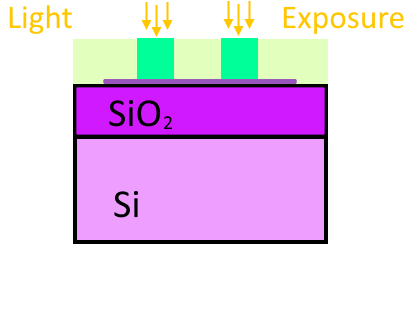
\includegraphics[width=\textwidth]{chap2/lithography/04Exposure}
		\caption{Masked exposure of photoresist to light}
	\end{subfigure}
	\end{figure}
	\begin{figure}[H]
	\centering
	\ContinuedFloat
	\begin{subfigure}{0.2\textwidth}
		\centering
		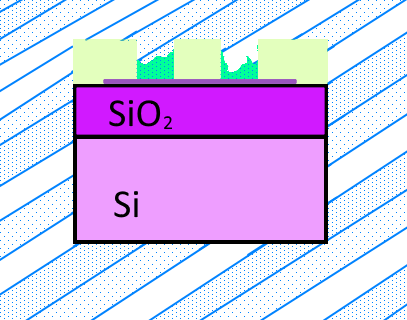
\includegraphics[width=\textwidth]{chap2/lithography/05Develop}
		\caption{Develop exposed photoresist}
	\end{subfigure}
	\hspace{0.04\textwidth}
	\begin{subfigure}{0.2\textwidth}
		\centering
		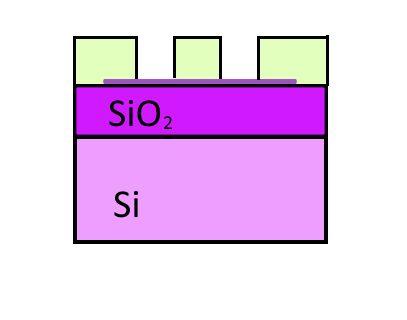
\includegraphics[width=\textwidth]{chap2/lithography/06Clean}
		\caption{Lithography structure}
	\end{subfigure}
	\hspace{0.04\textwidth}
	\begin{subfigure}{0.2\textwidth}
		\centering
		
\includegraphics[width=\textwidth]{placeholder}
		\caption{UV Ozone Cleaning}
	\end{subfigure}
	\hspace{0.04\textwidth}
	\begin{subfigure}{0.2\textwidth}
		\centering
		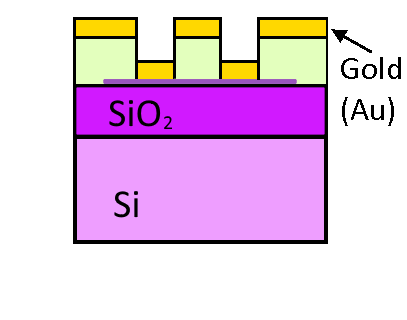
\includegraphics[width=\textwidth]{chap2/lithography/07Deposition}
		\caption{Deposition of metals}
	\end{subfigure}
	\end{figure}
	\begin{figure}[H]
	\ContinuedFloat
	\centering
	\begin{subfigure}{0.2\textwidth}
		\centering
		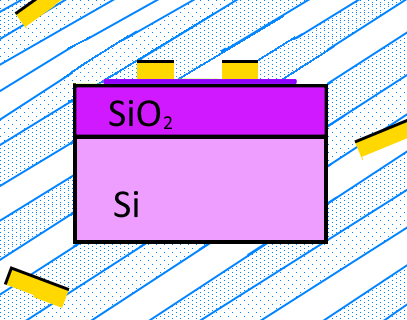
\includegraphics[width=\textwidth]{chap2/lithography/07LiftOff}
		\caption{Lift off: Removal of remaining photoresist and excess metal}
	\end{subfigure}
	\hspace{0.04\textwidth}
	\begin{subfigure}{0.2\textwidth}
		\centering
		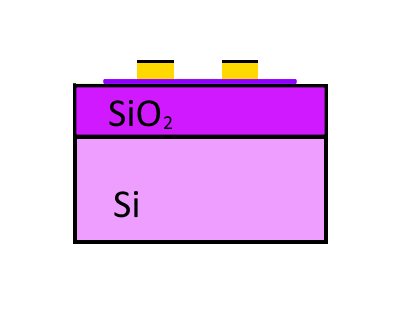
\includegraphics[width=\textwidth]{chap2/lithography/08Clean}
		\caption{Final result}
	\end{subfigure}
	\caption{Device fabrication process}\label{fig:litho}
	From exfoliated graphene to a FET.
	\end{figure}
	
	\subsection{Exfoliation}\label{sec:exfoliation}
	Exfoliation in materials refers to the cleaving thin layers (or leaves) off a larger sample, and acquiring them onto the substrate. We exfoliate graphene onto Si/SiO$_2$ wafers.
	Exfoliation can take a variety of forms, from Geim's method \cite{novoselov_two-dimensional_2005}, to directly applying scotch tape to HOPG and then pressing against SiO$_2$, before peeling the tape off. 
	
	Huang \etal investigated a reliable method of exfoliation to produce large area and high quality samples \cite{huang_reliable_2015}, which has been widely cited. Tape with graphite flakes is brought into contact with a silicon dioxide wafer, and an annealing process of heating the tape and wafer for 2-5m at $\sim 100^\circ$C on a conventional lab hot plate is used. After allowing cooling to room temperature, the tape is removed. They find under optical microscopy that graphene flakes with uniform thickness routinely range from $\sim 20\mu$m to above $100\mu$m. In this context, annealing is expected to increase traction due to the remove of gas moelcules trapped between SiO$_2$ and graphite.\newline 
	
	The following steps make up the process of exfoliation we optimised:
	\begin{enumerate}
		\itemsep 0em
		\item (Optional) Use a plasma asher/etcher with an argon/oxygen plasma to the clean surface of \silicondioxide. This can increase the adhesion between graphene and the surface by removing organic absorbates\cite{huang_reliable_2015}. Alternatively, clean wafers of Si/SiO$_2$ in acetone, tilted in an ultrasonic bath for 30s. Repeat the same in isopropanol, before rinsing in ethanol and drying with N$_2$ gas.
		\item Cleave a layer of HOPG graphite by using scotch tape to peel off a thick film.
		\item Use a secondary piece of scotch tape to exfoliate a thinner layer off master tape. Ensure good coverage by reattaching a couple times. 
		\item Attach Si/SiO$_2$ wafers to graphite covered areas of secondary tape. The SiO$_2$ face should be contacting the graphite.
		\item Attach the tape and wafers firmly to a glass slide, before using a tissue/cotton-bud to press the surface of the tape into the wafer.
		\item Place glass slide on a hotplate at $100^\circ$C for two minutes, before removing and cooling for two minutes.
		\item Slowly peel tape at an acute angle from the glass slide, roughly at 6s per cm over the wafer.
	\end{enumerate}
	
	We found success can depend on HOPG crystal, given we tried cleavage using ZYA and ZYB quality crystals and had repeated failure. Changing to a new ZYA crystal provided immediate results using the same process.
	
	\subsection{Lithography}\label{sec:lithography}
	Lithography can be used to create polymer structures that allow the deposition of desired material in 2D geometries. This is used to create electrical contacts onto graphene. This process and the adjustements made for fabricating our devices are described in this section.\newline
	
	Lithography typically consists of three main steps.
	\begin{enumerate}
		\itemsep0em
		\item Spin coating - covering a sample with a uniform layer of polymer, and baking it on.
		\item Exposure - The polymer undergoes chemical changes to its properties when exposed to particular wavelengths of light. This differentiates exposed areas to those unexposed.
		\item Developer solution - developer solution removes indended areas of photoresist to create structures.
	\end{enumerate}
	
	\subsubsection{Spin coating photoresists}\label{sec:resists}
	A spin coater is used to deposit thin films of materials. A vacuum holds a sample on the spinner, before drops of photoresist are introduced to the sample, which is then spun over sometime to achieve a uniform thickness of photoresist. Baking on a hotplate follows to set the photoresist layer on the sample.
	
	Photoresists vary in their spinning thickness, but also their exposure rates. Positive photoresists dissolve in particular developer solutions when exposed to light, while negative photoresists dissolve if not exposed to light. We have only used positive photoresists, as we have primarily been creating structures for deposition, and not etching material where you want the bulk of the wafer exposed.
	
	\paragraph{HMDS \& AZ-1512HS}
	Initially devices were fabricated using the AZ-1512HS polymer, with the additional use of hexamethyldisilazane (HMDS) as an adhesion promoter between SiO$_2$ and AZ-1512HS. Devices were spun initially for 10 s at 1000 rpm, before being spun between 2000 and 3000 rpm for 30 s, per resist layer. This leaves a thickness of 1.7 $\mu$m to 1.39 $\mu$m \cite{az1500_series}.
	Devices were then baked at 100 $^\circ$C for 1 minute.
	
	\begin{figure}[H]\label{fig:spin_curve_AZ-1512HS}
		\centering
		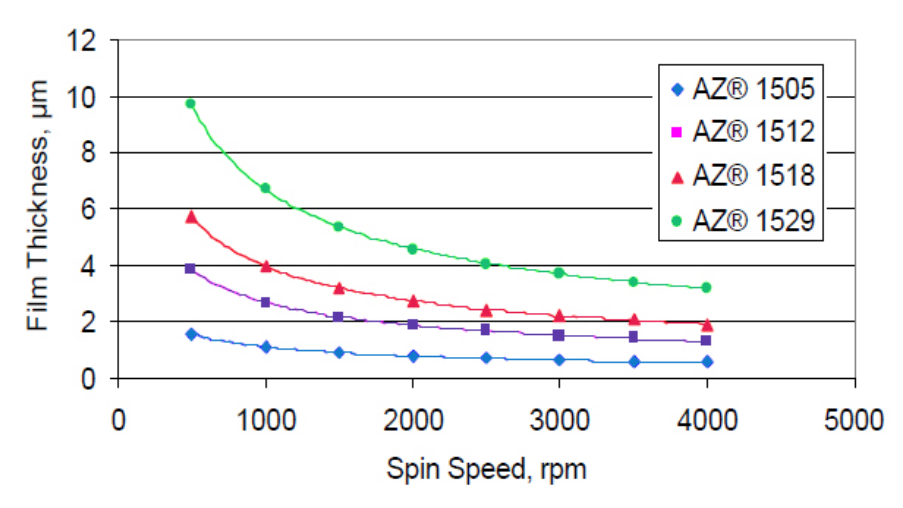
\includegraphics[width=0.7\textwidth]{chap2/az1512-spin-curve.png}
		\caption{Spin curve of AZ-1512HS (Source: EMD Performance Materials\cite{az1500_series_spincurve})}
	\end{figure}
	
	\paragraph{Skin issues with HMDS}\label{sec:sin_issues}
	When using HMDS and AZ-1512HSHS in conjunction, significant amounts of deposition remenants were found on samples as seen in \cref{fig:lithography_skins}.
	
	\begin{figure}[H]
		\centering
		\begin{subfigure}[b]{0.3\textwidth}
			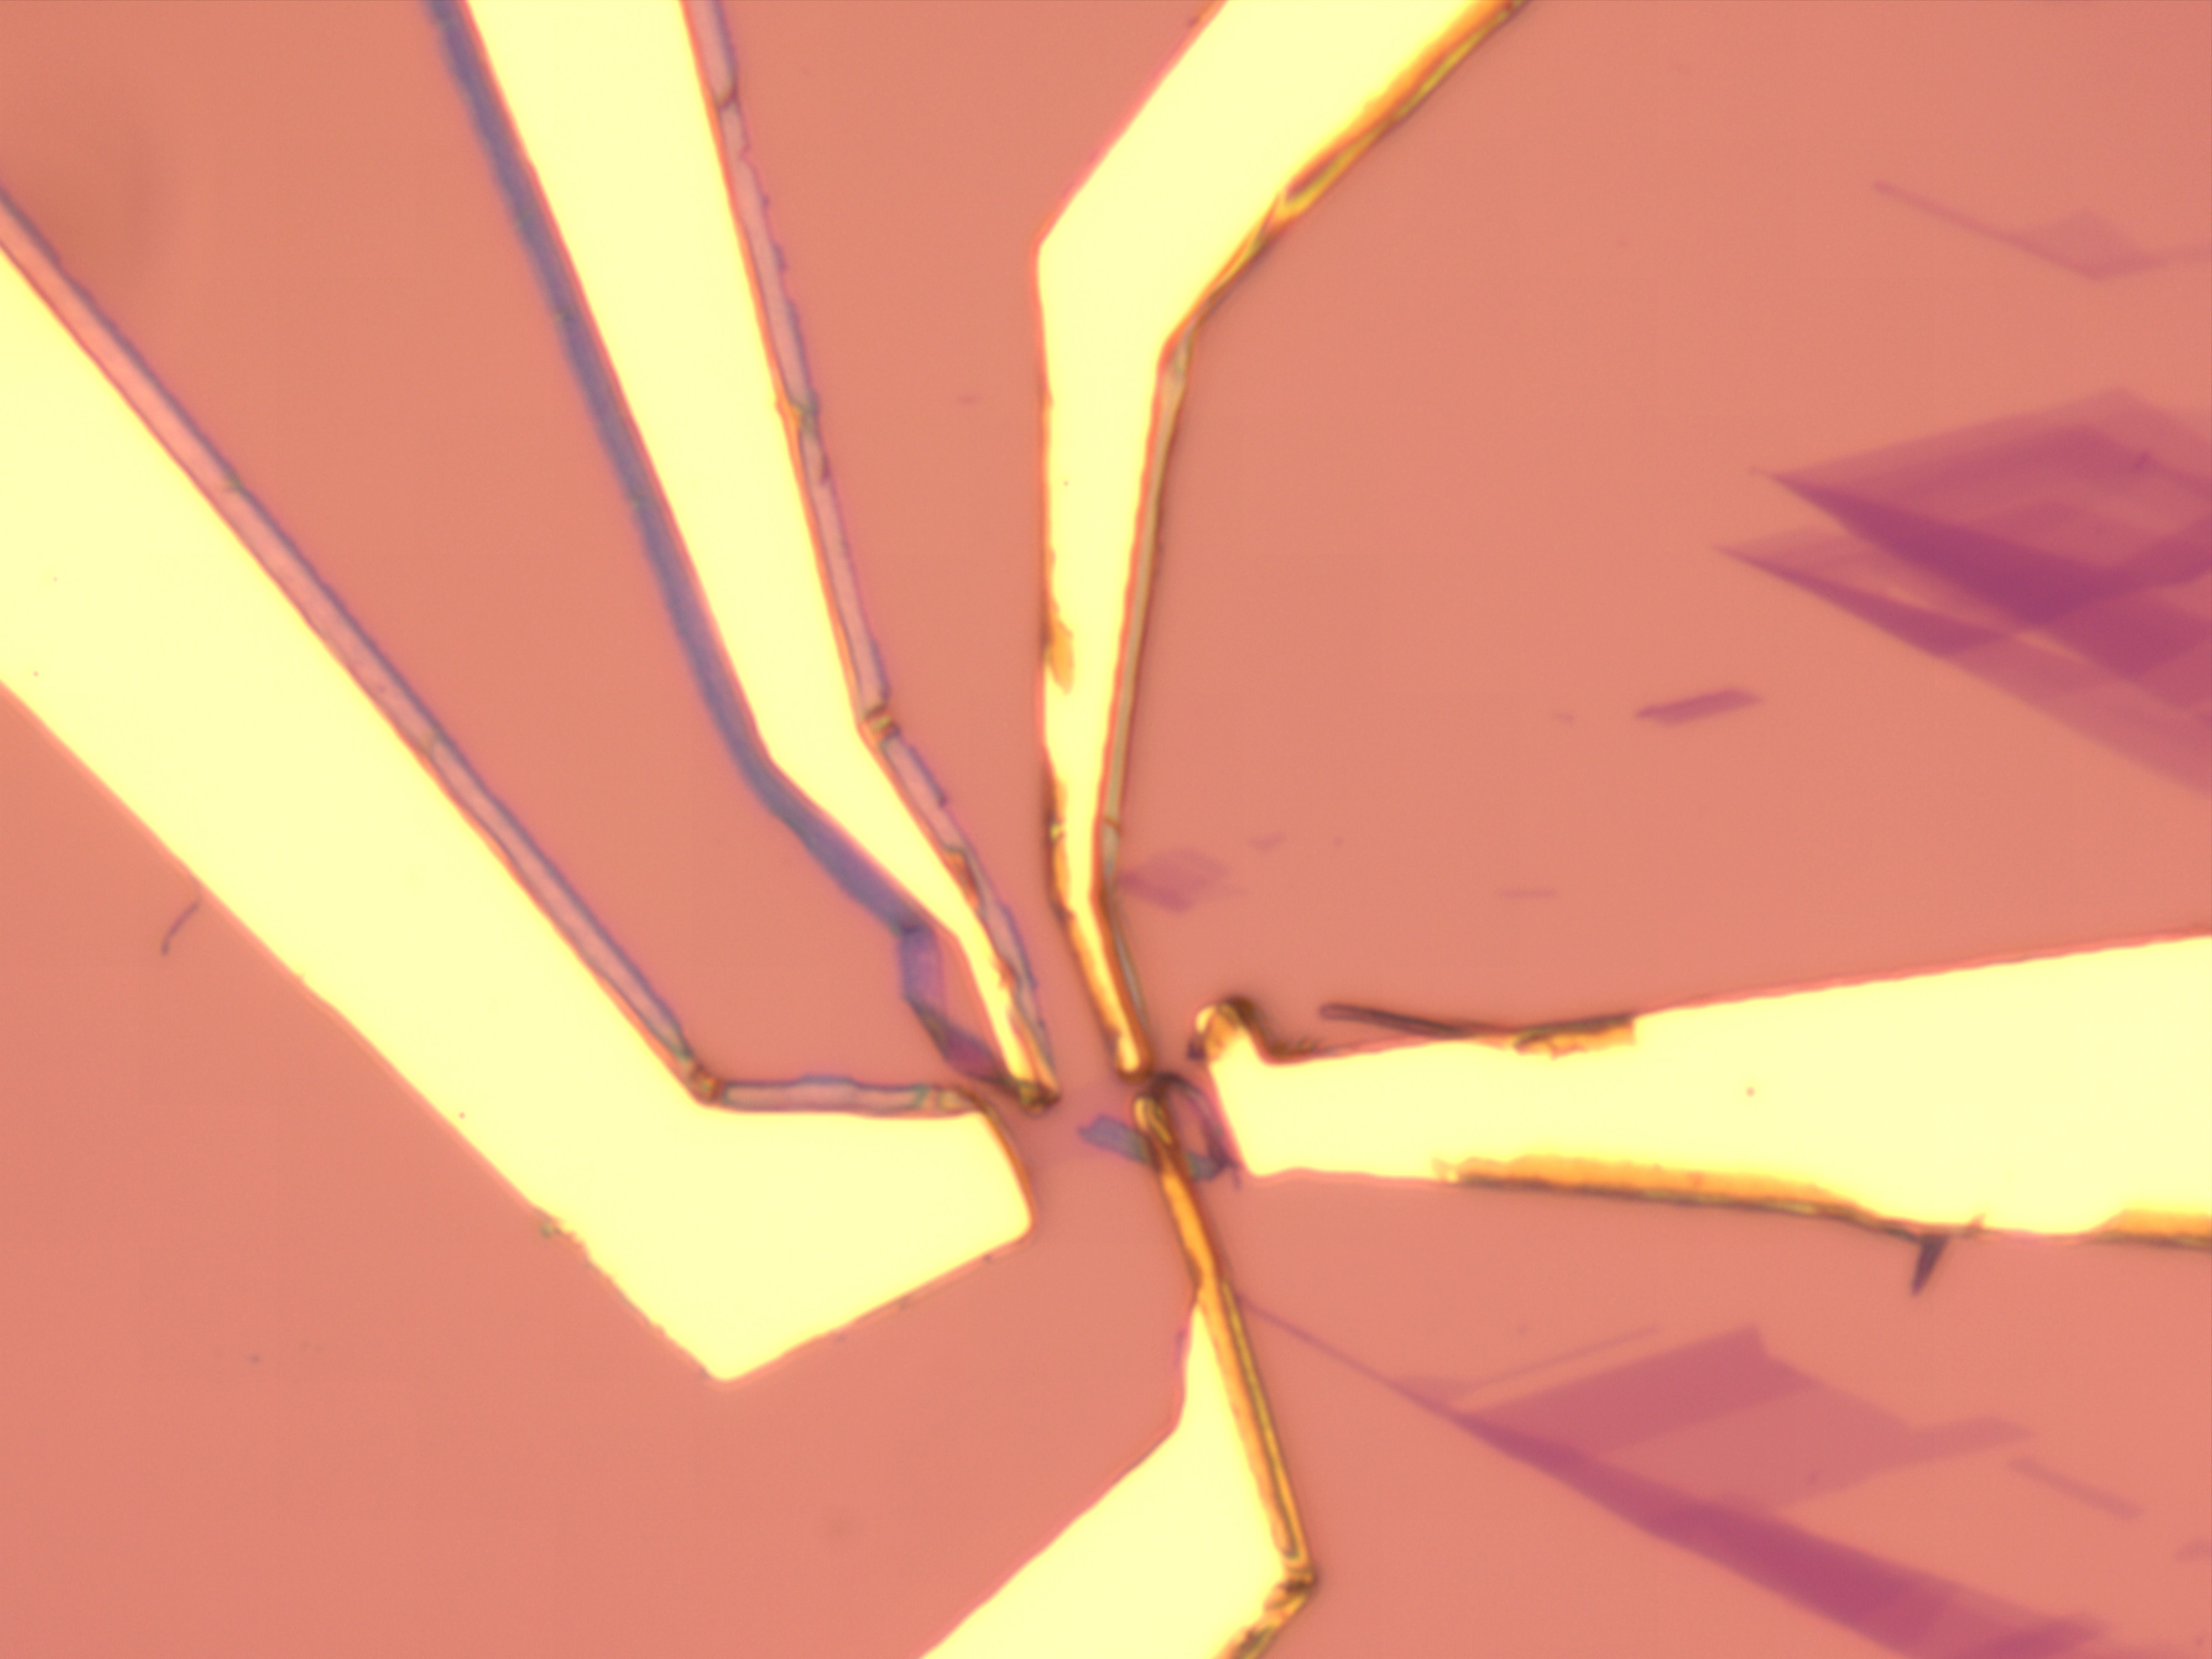
\includegraphics[width=\textwidth]{chap2/skins/Litho01_B07_WA1_F10_100x.jpg}
%			\caption{}
		\end{subfigure}
		\begin{subfigure}[b]{0.3\textwidth}
			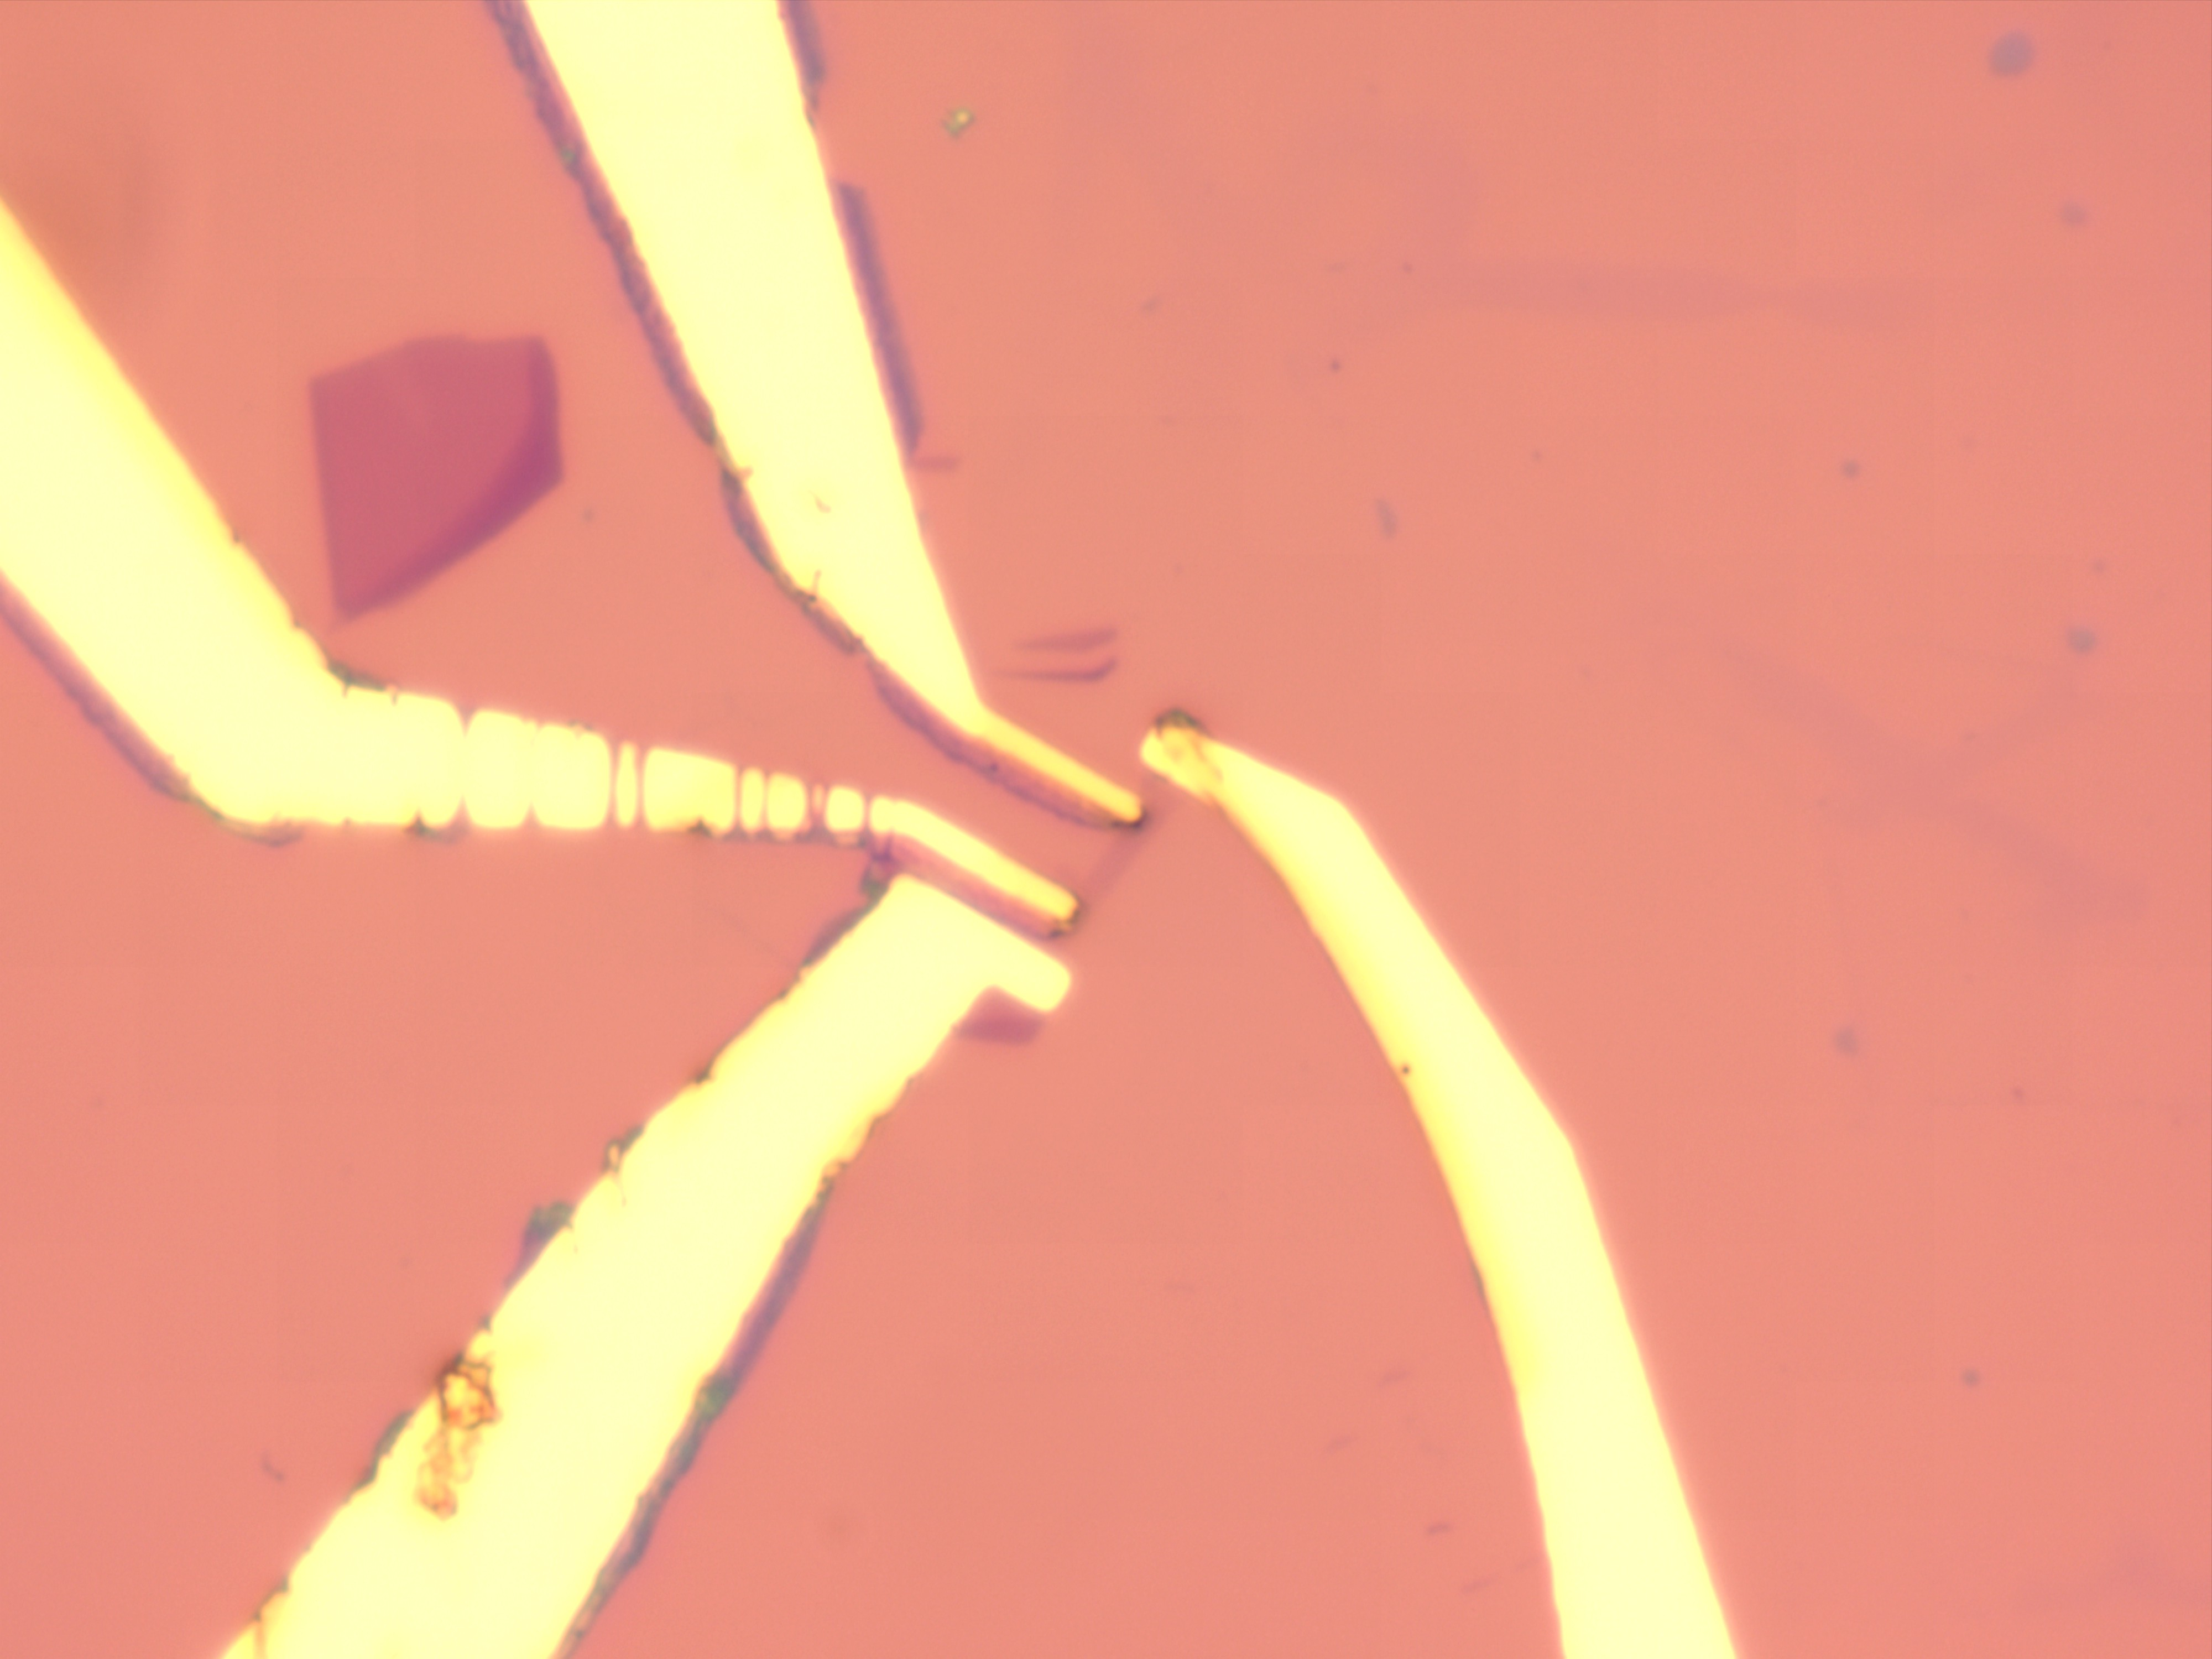
\includegraphics[width=\textwidth]{chap2/skins/1_100x.jpg}
%			\subcaption{}
		\end{subfigure}
		\begin{subfigure}[b]{0.3\textwidth}
			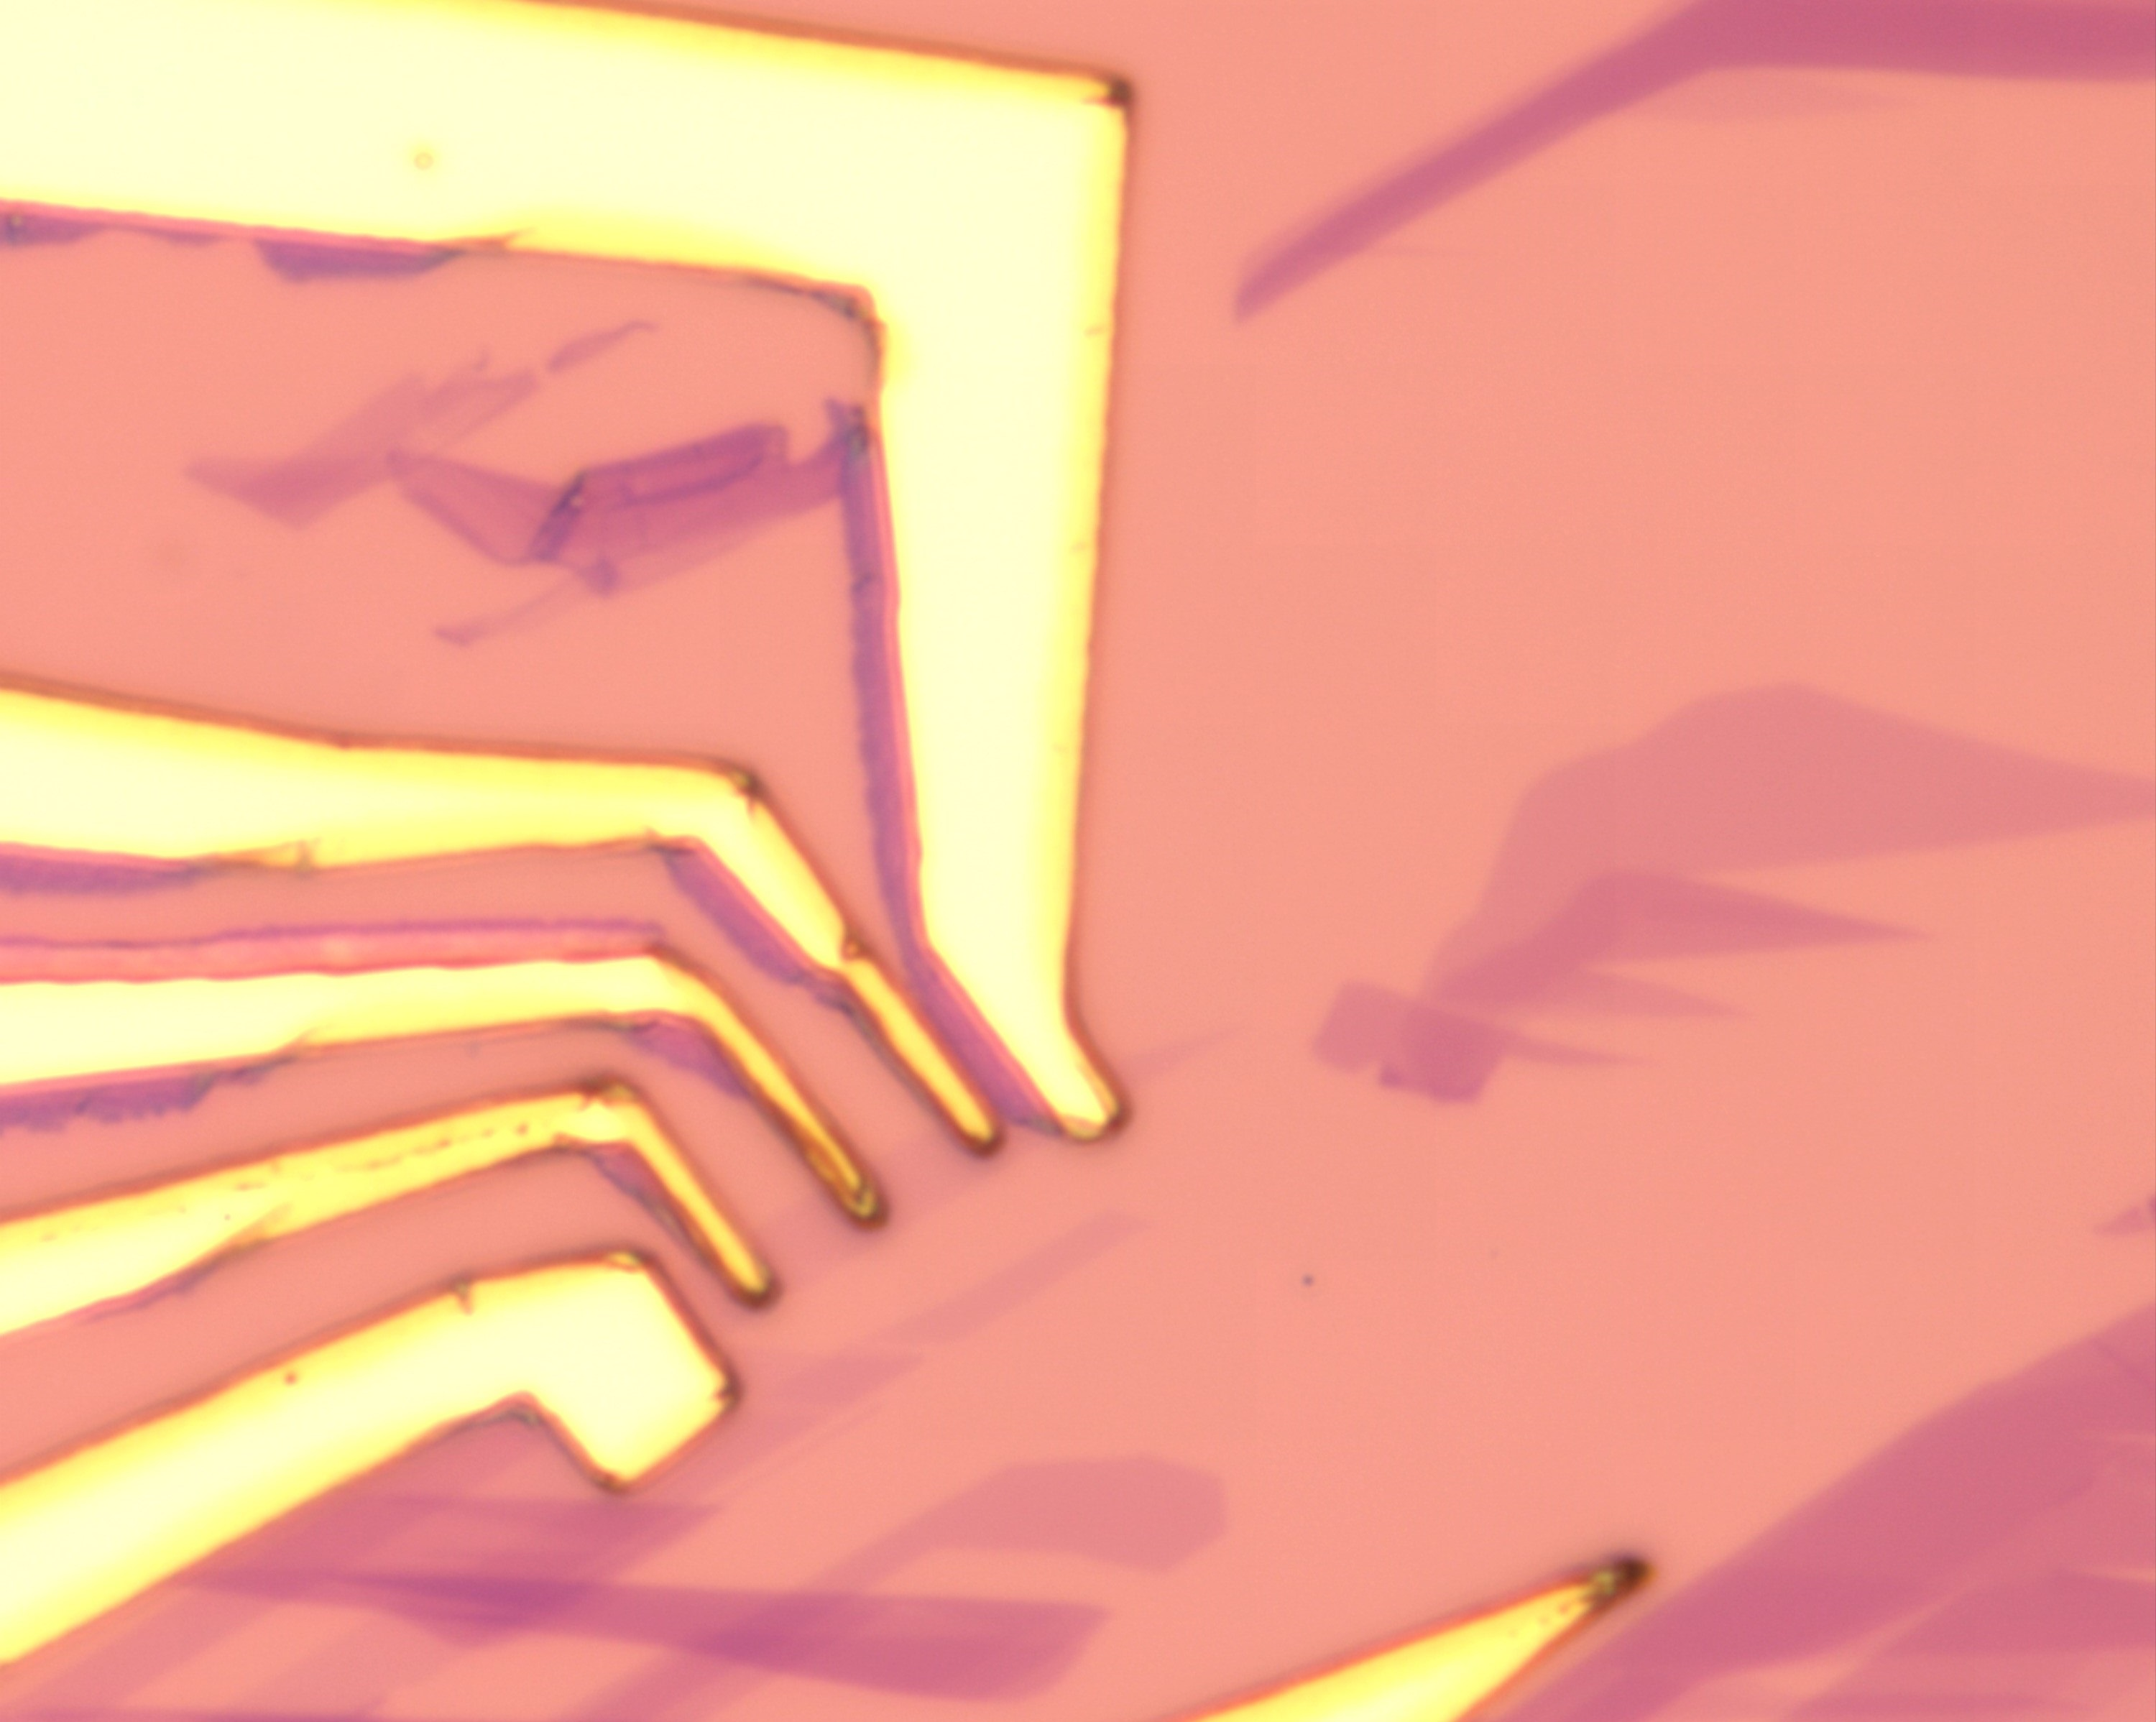
\includegraphics[width=\textwidth]{chap2/skins/2_100x_v2.jpg}
%			\subcaption{after 10s ultrasonication}		
		\end{subfigure}
		\caption{Material remanants from lithography. Gold edges exhibit a bluish remnant edge.}\label{fig:lithography_skins}
		%TODO orientate images, and update examples.
	\end{figure}
	
	This is likely due to metal deposition (ie, Chromium, see \cref{sec:deposition}) forming layers on the sides of lithography wells, as the skins have very similar geometry to that of either the wells or the edges. The spinning speeds give resist heights (ie, the well edge heights) roughly the same as feature width ($\approx$1$\mu$m minimum), matching the observed result.
	
	Sometimes these remenants could be cleaned off, through the use of ultrasonication, however this had a large risk of damaging the graphene, seen in \cref{fig:lithography_skins_break}.
	
	\begin{figure}[H]
		\centering
		\begin{subfigure}[b]{0.3\textwidth}
			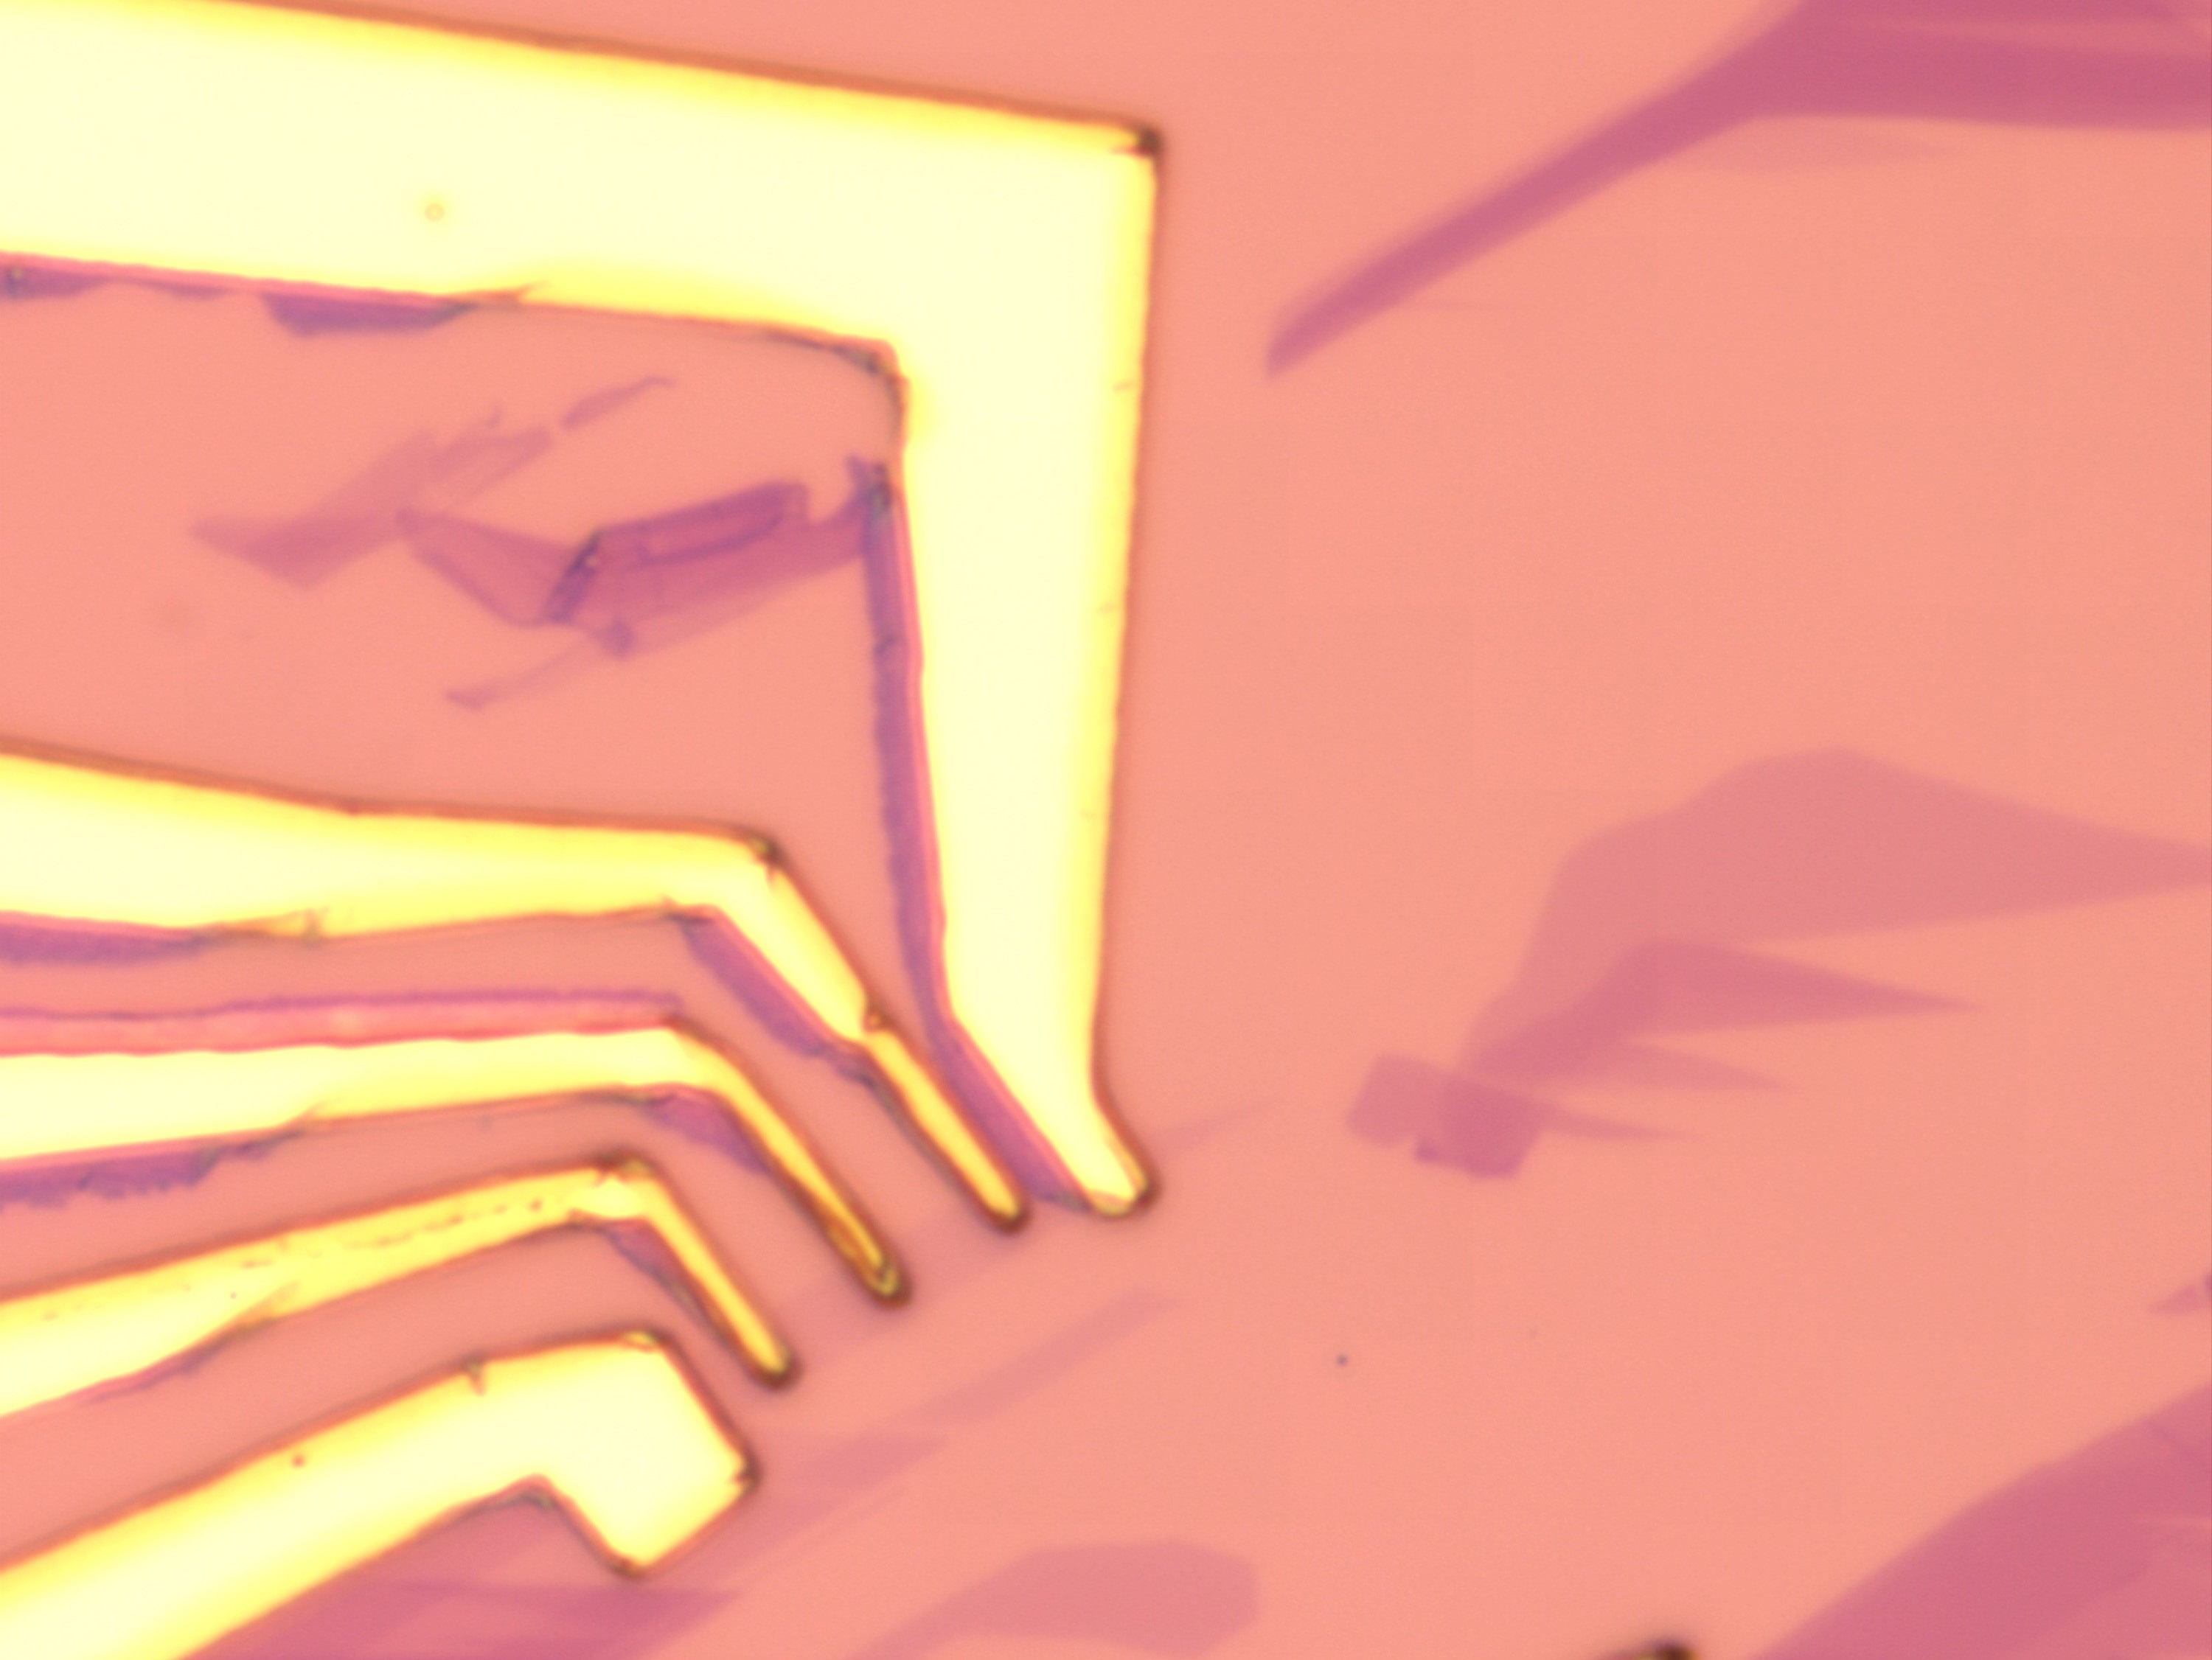
\includegraphics[width=\textwidth]{chap2/US/2_100x.jpg}
			\caption{After metal lift off}			
		\end{subfigure}
		\begin{subfigure}[b]{0.3\textwidth}
			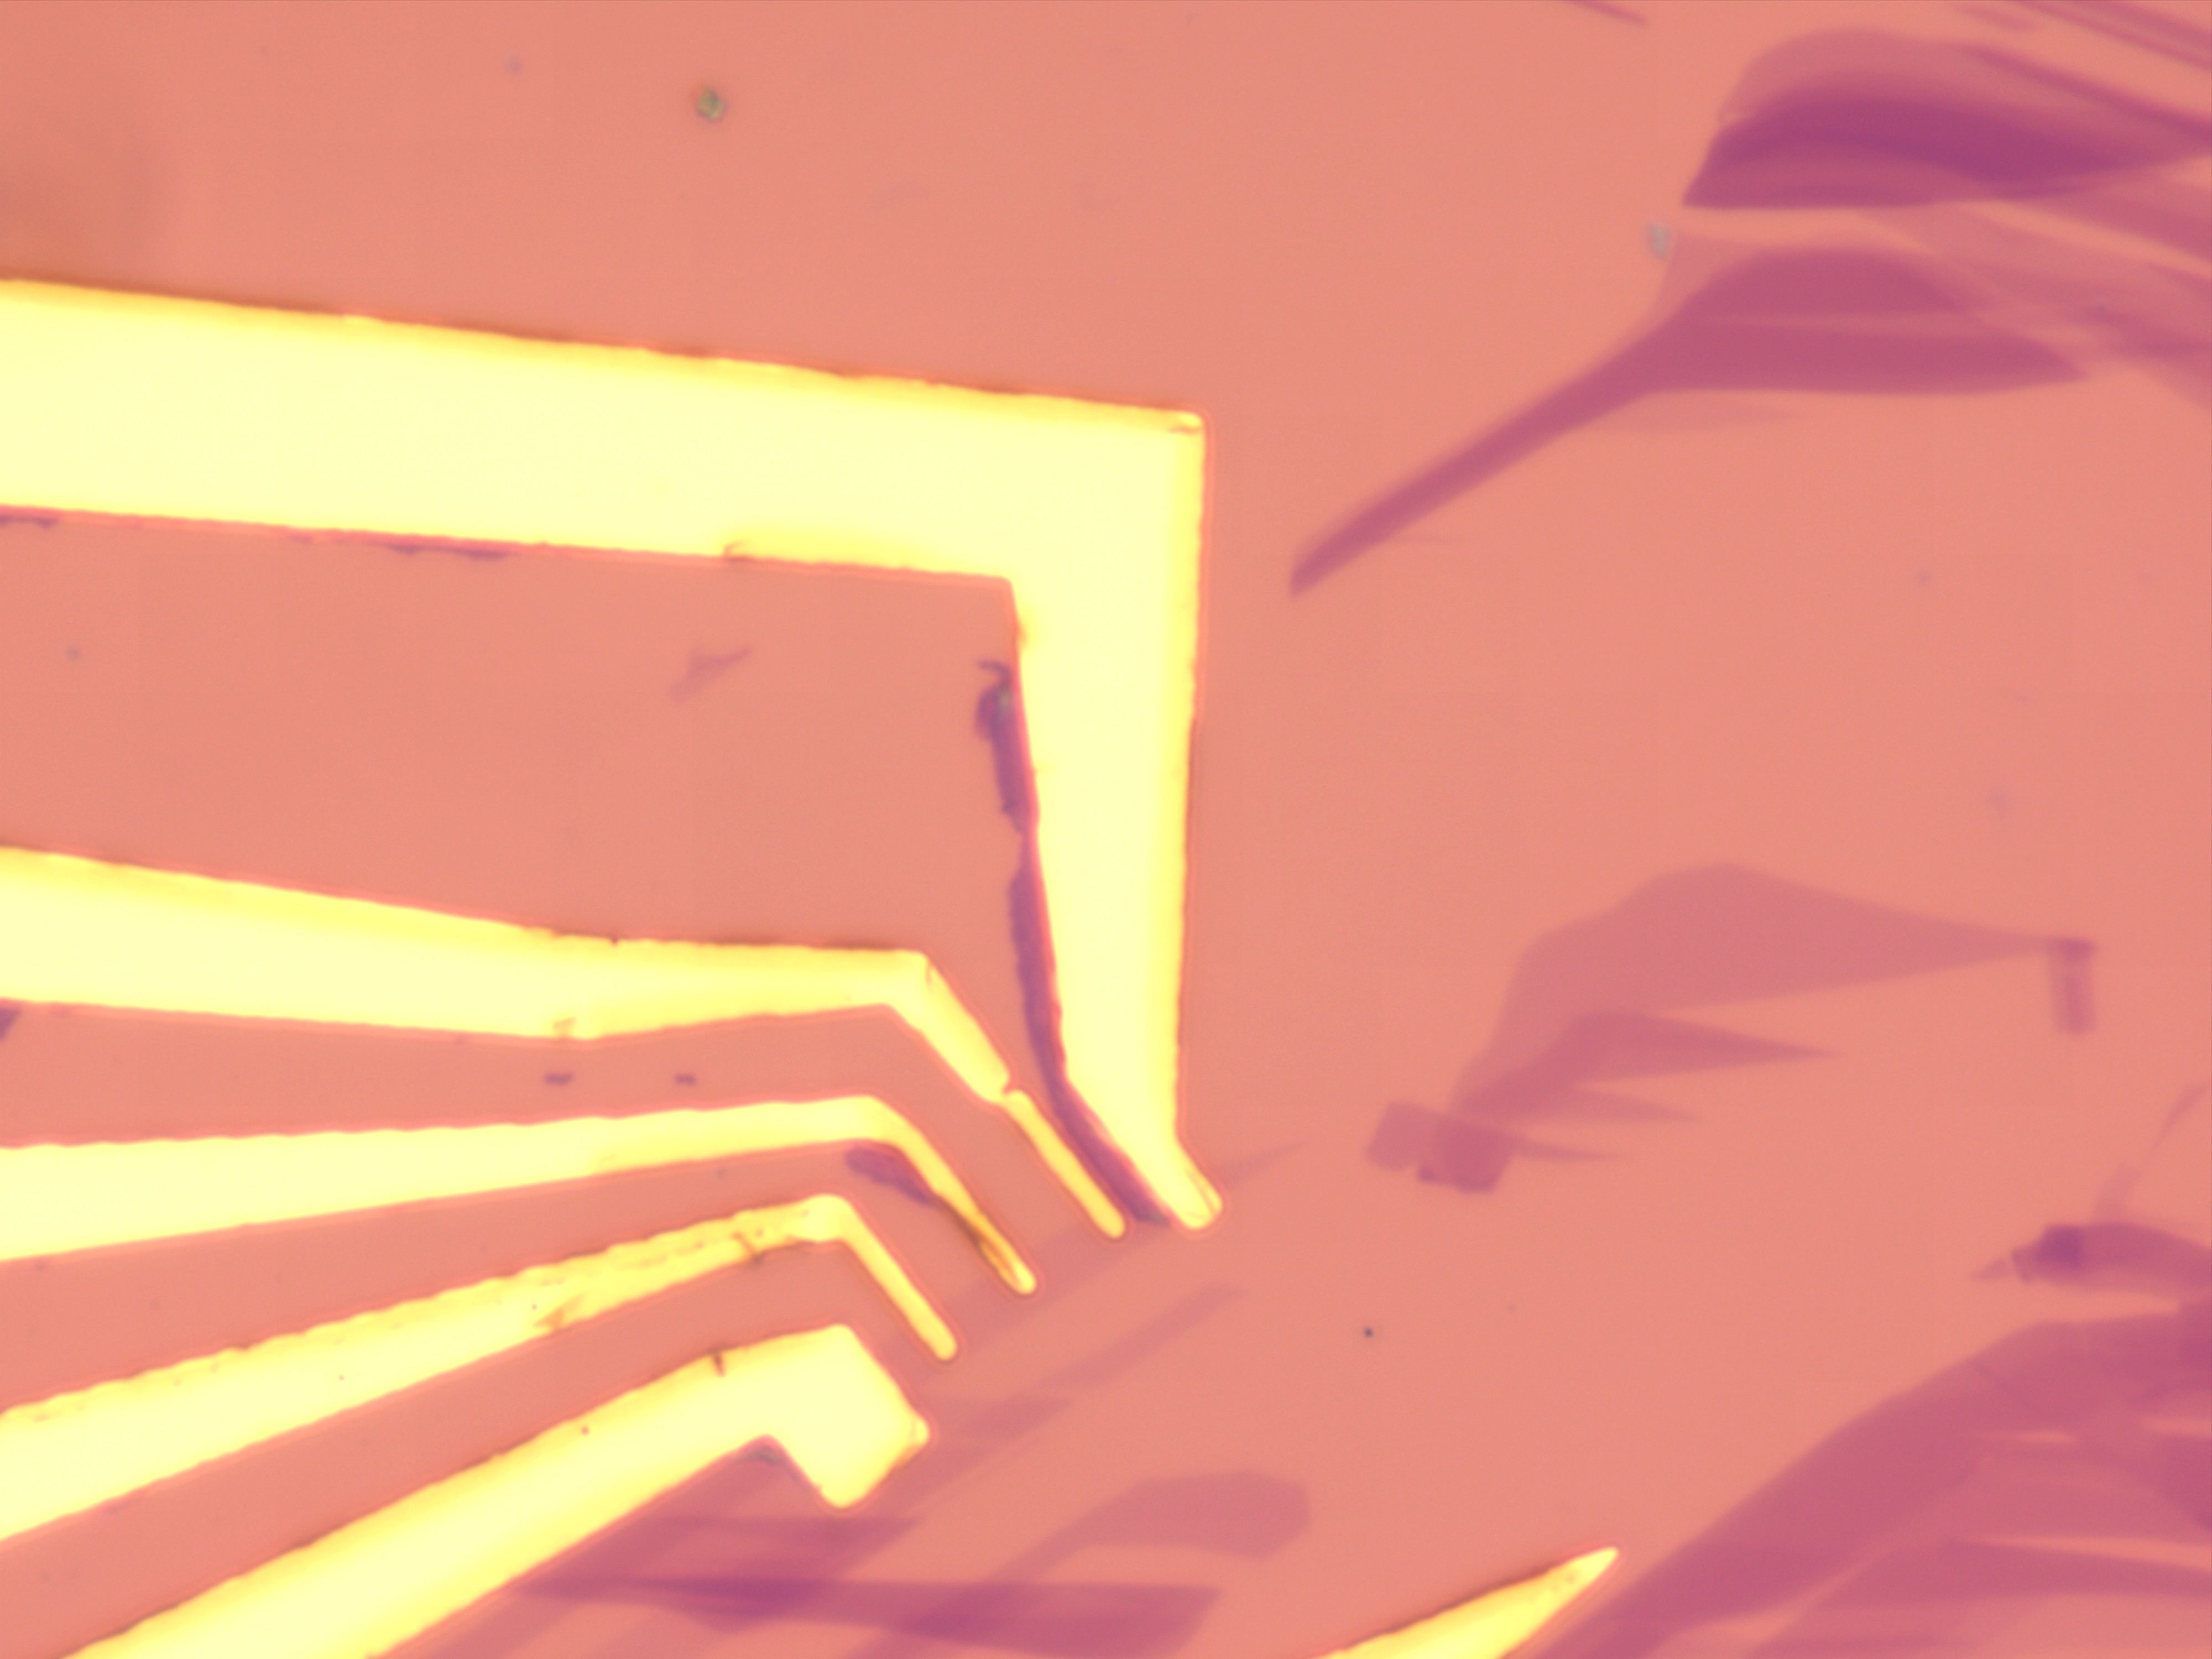
\includegraphics[width=\textwidth]{chap2/US/2_100x_after6sAcetoneUS.jpg}
			\subcaption{after 5s ultrasonication}
		\end{subfigure}
		\begin{subfigure}[b]{0.3\textwidth}
			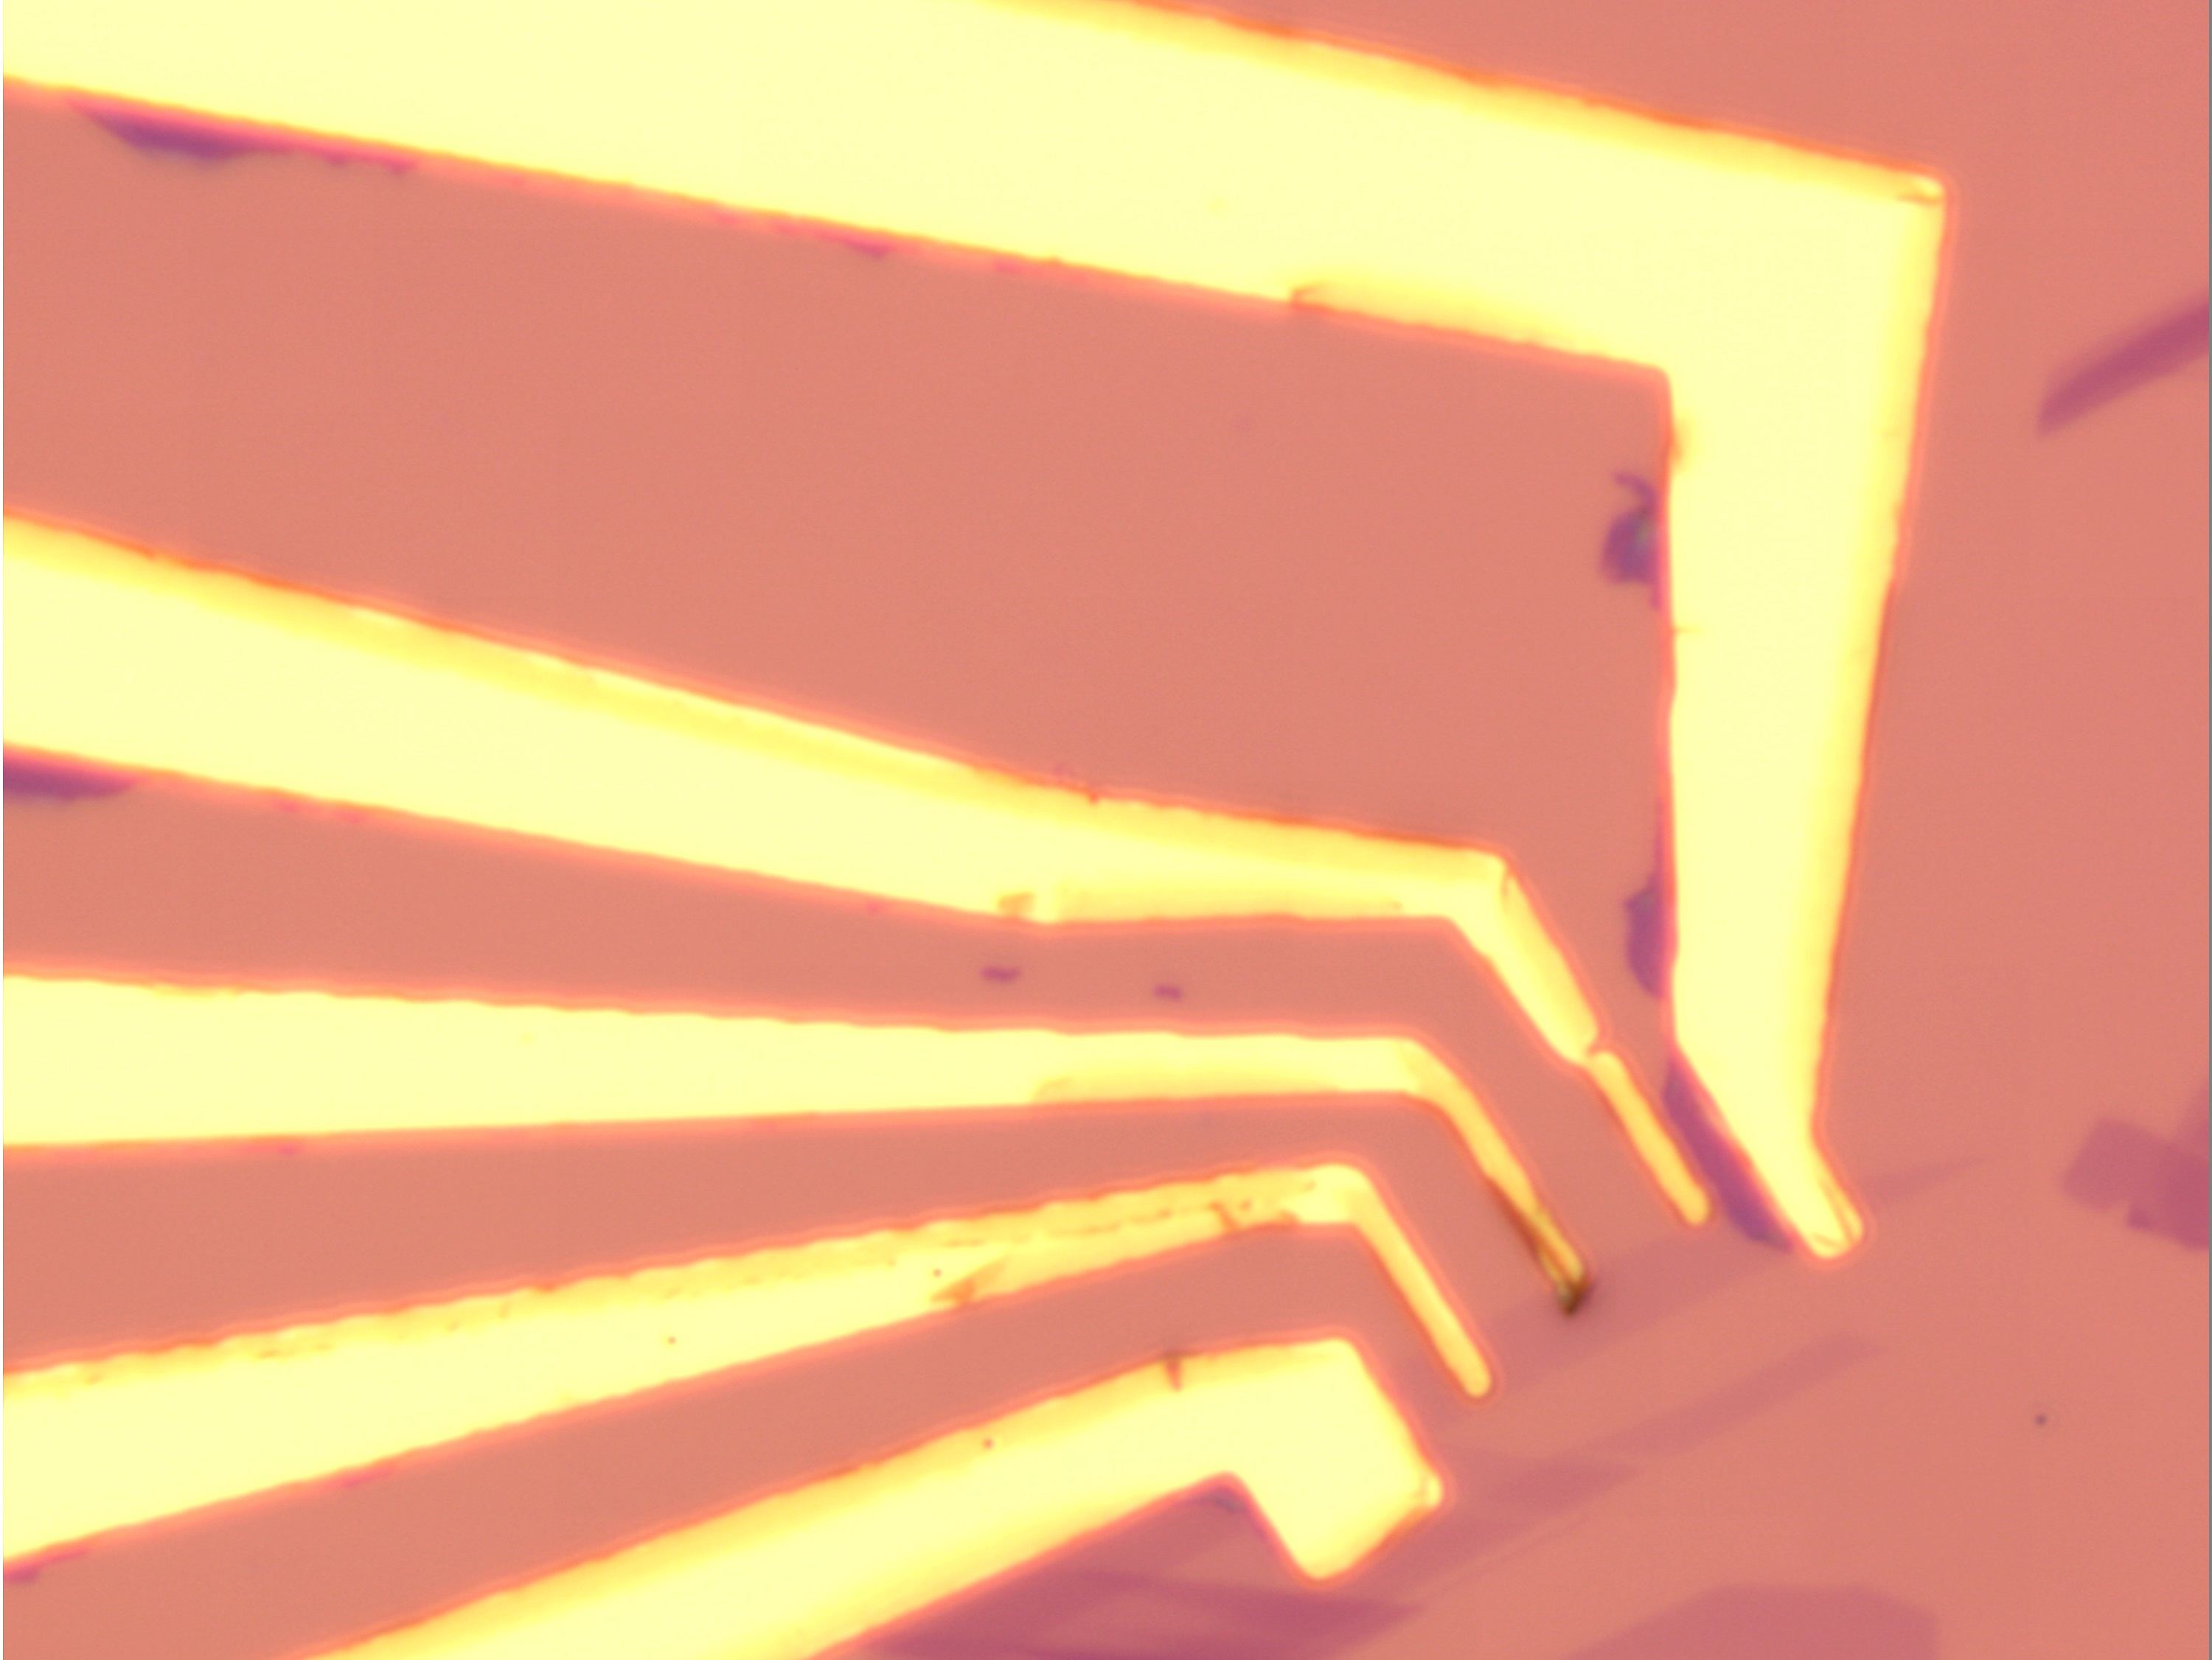
\includegraphics[width=\textwidth]{chap2/US/2_100x_after10sAcetoneUS.jpg}
			\subcaption{after 10s ultrasonication}		
		\end{subfigure}
		\caption{Ultrasonication used to remove material remanants from lithography.}\label{fig:lithography_skins_us}Note the movement or loss of gold material on the middle probes.
	\end{figure}

	\begin{figure}[H]
		\centering
		\begin{subfigure}[b]{0.3\textwidth}
			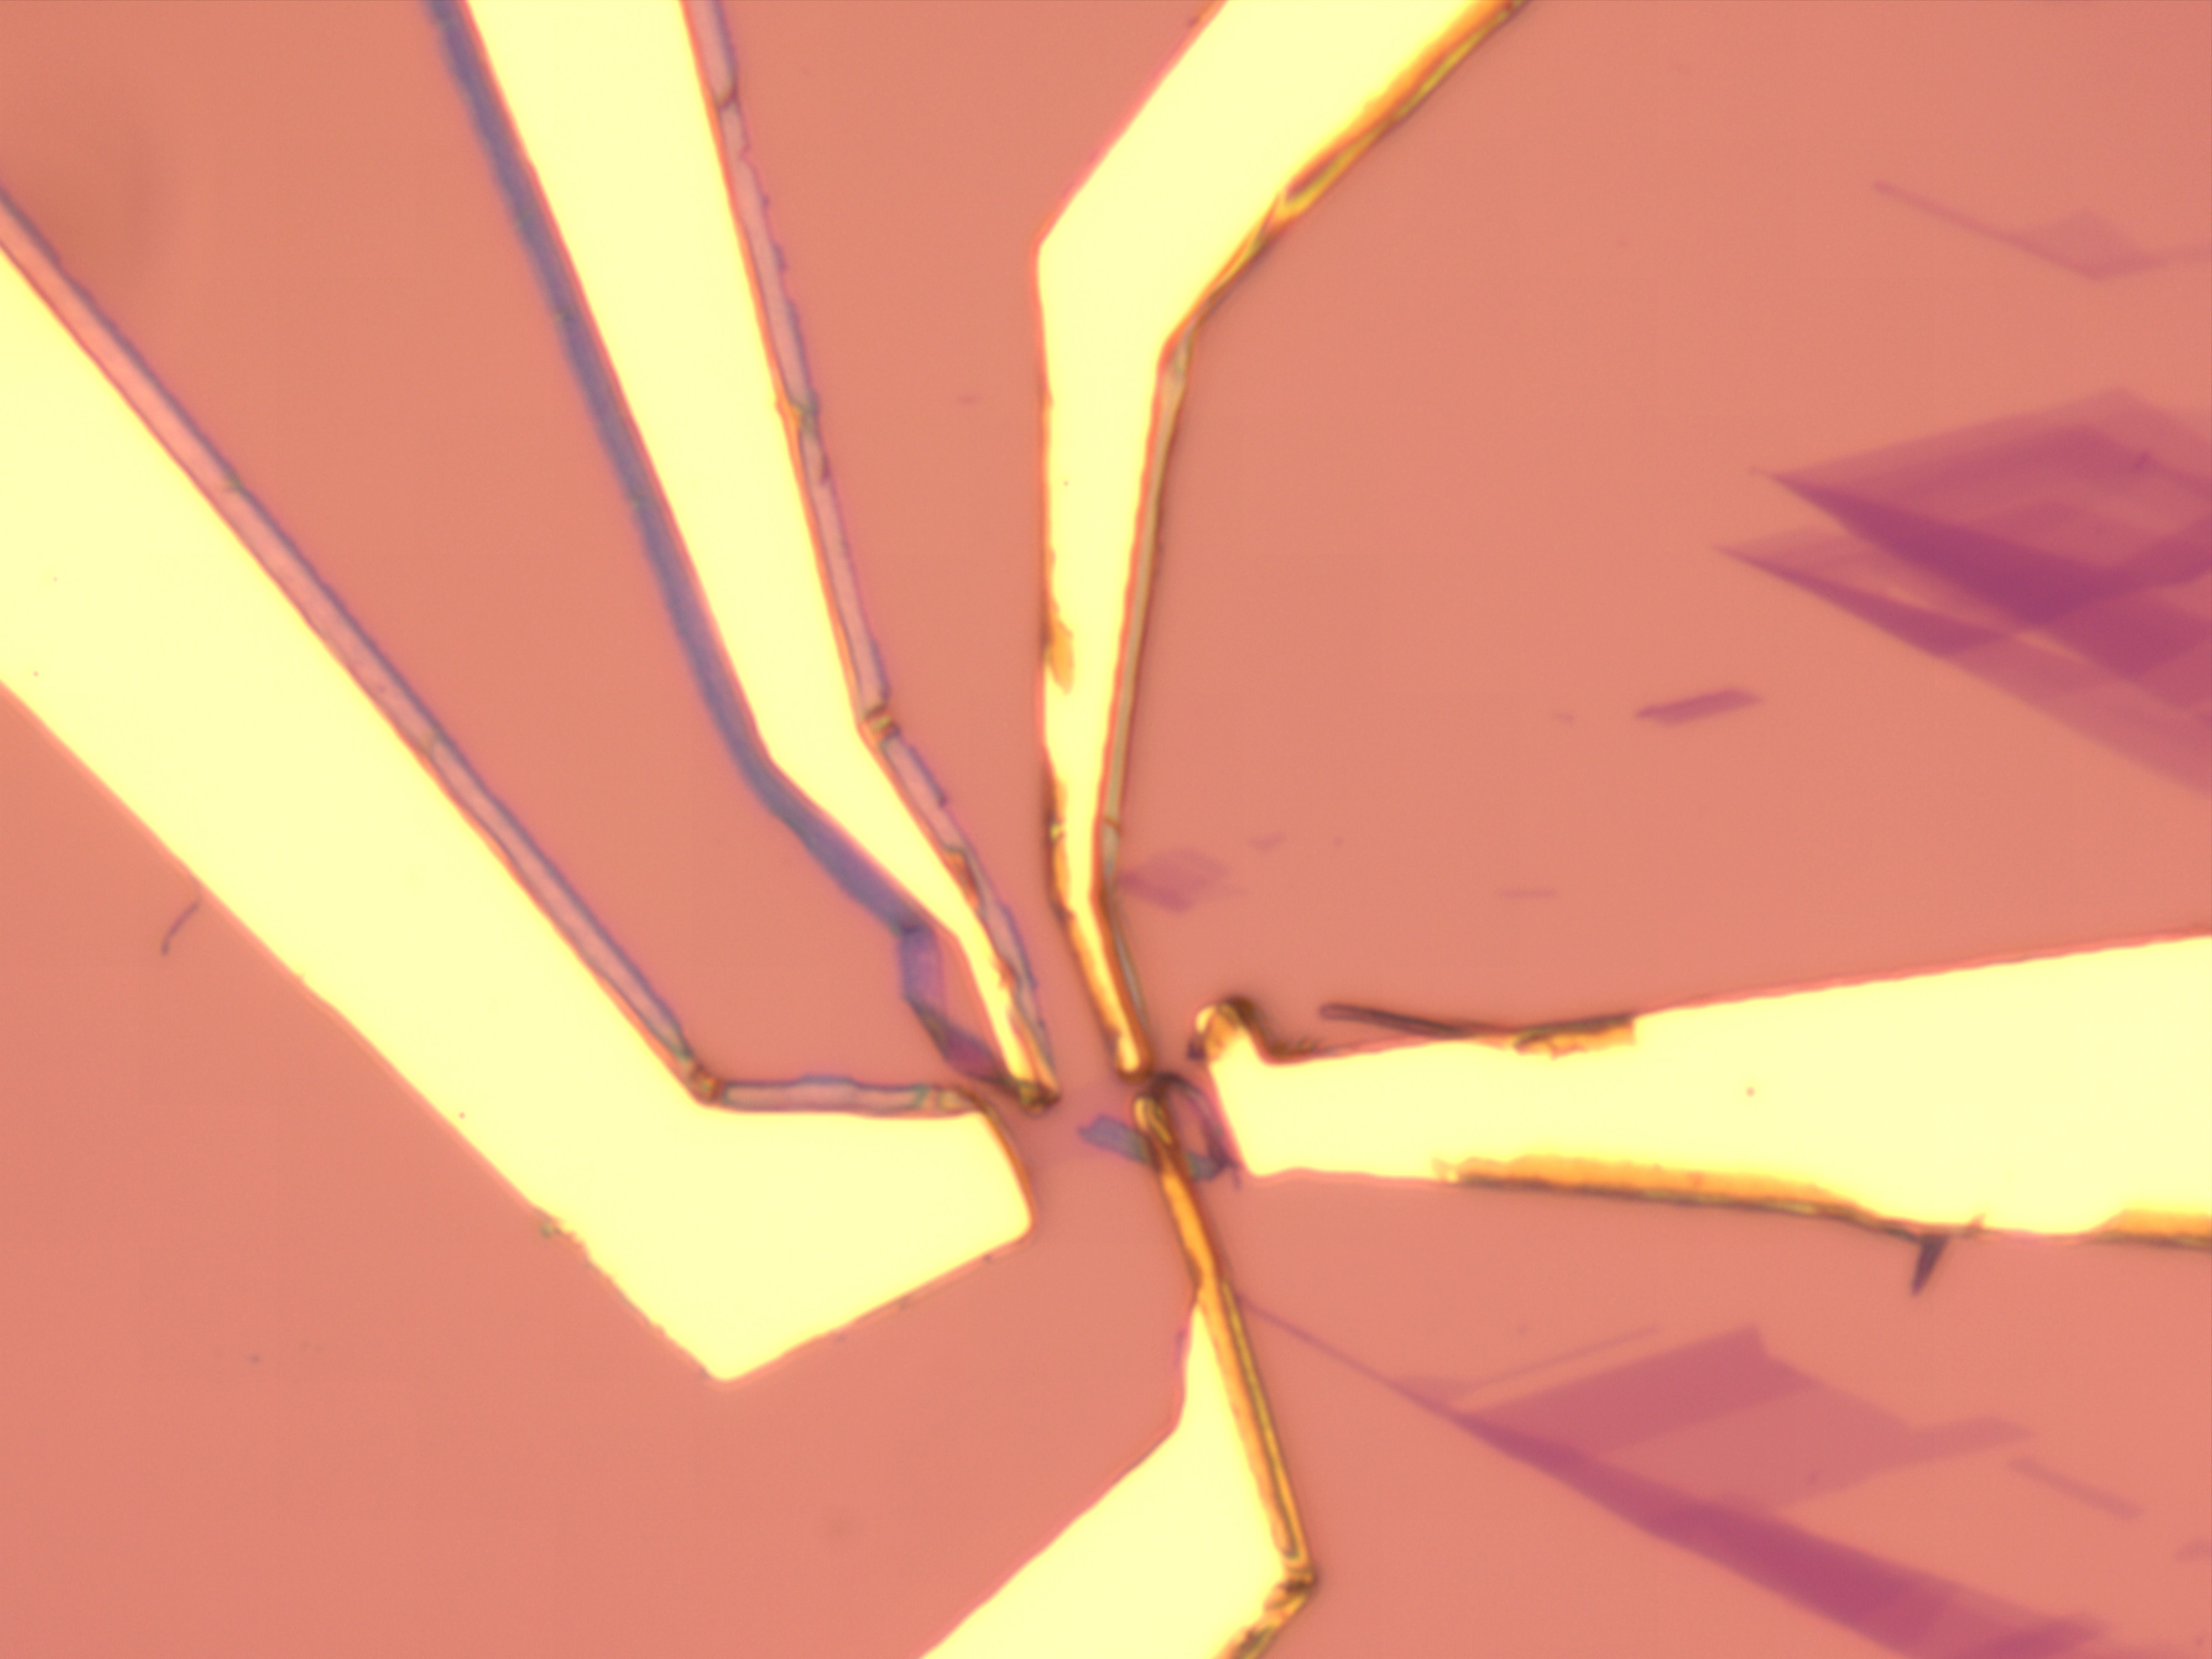
\includegraphics[width=\textwidth]{chap2/US/1_a}
			\caption{After metal lift off}
		\end{subfigure}
		\begin{subfigure}[b]{0.3\textwidth}
			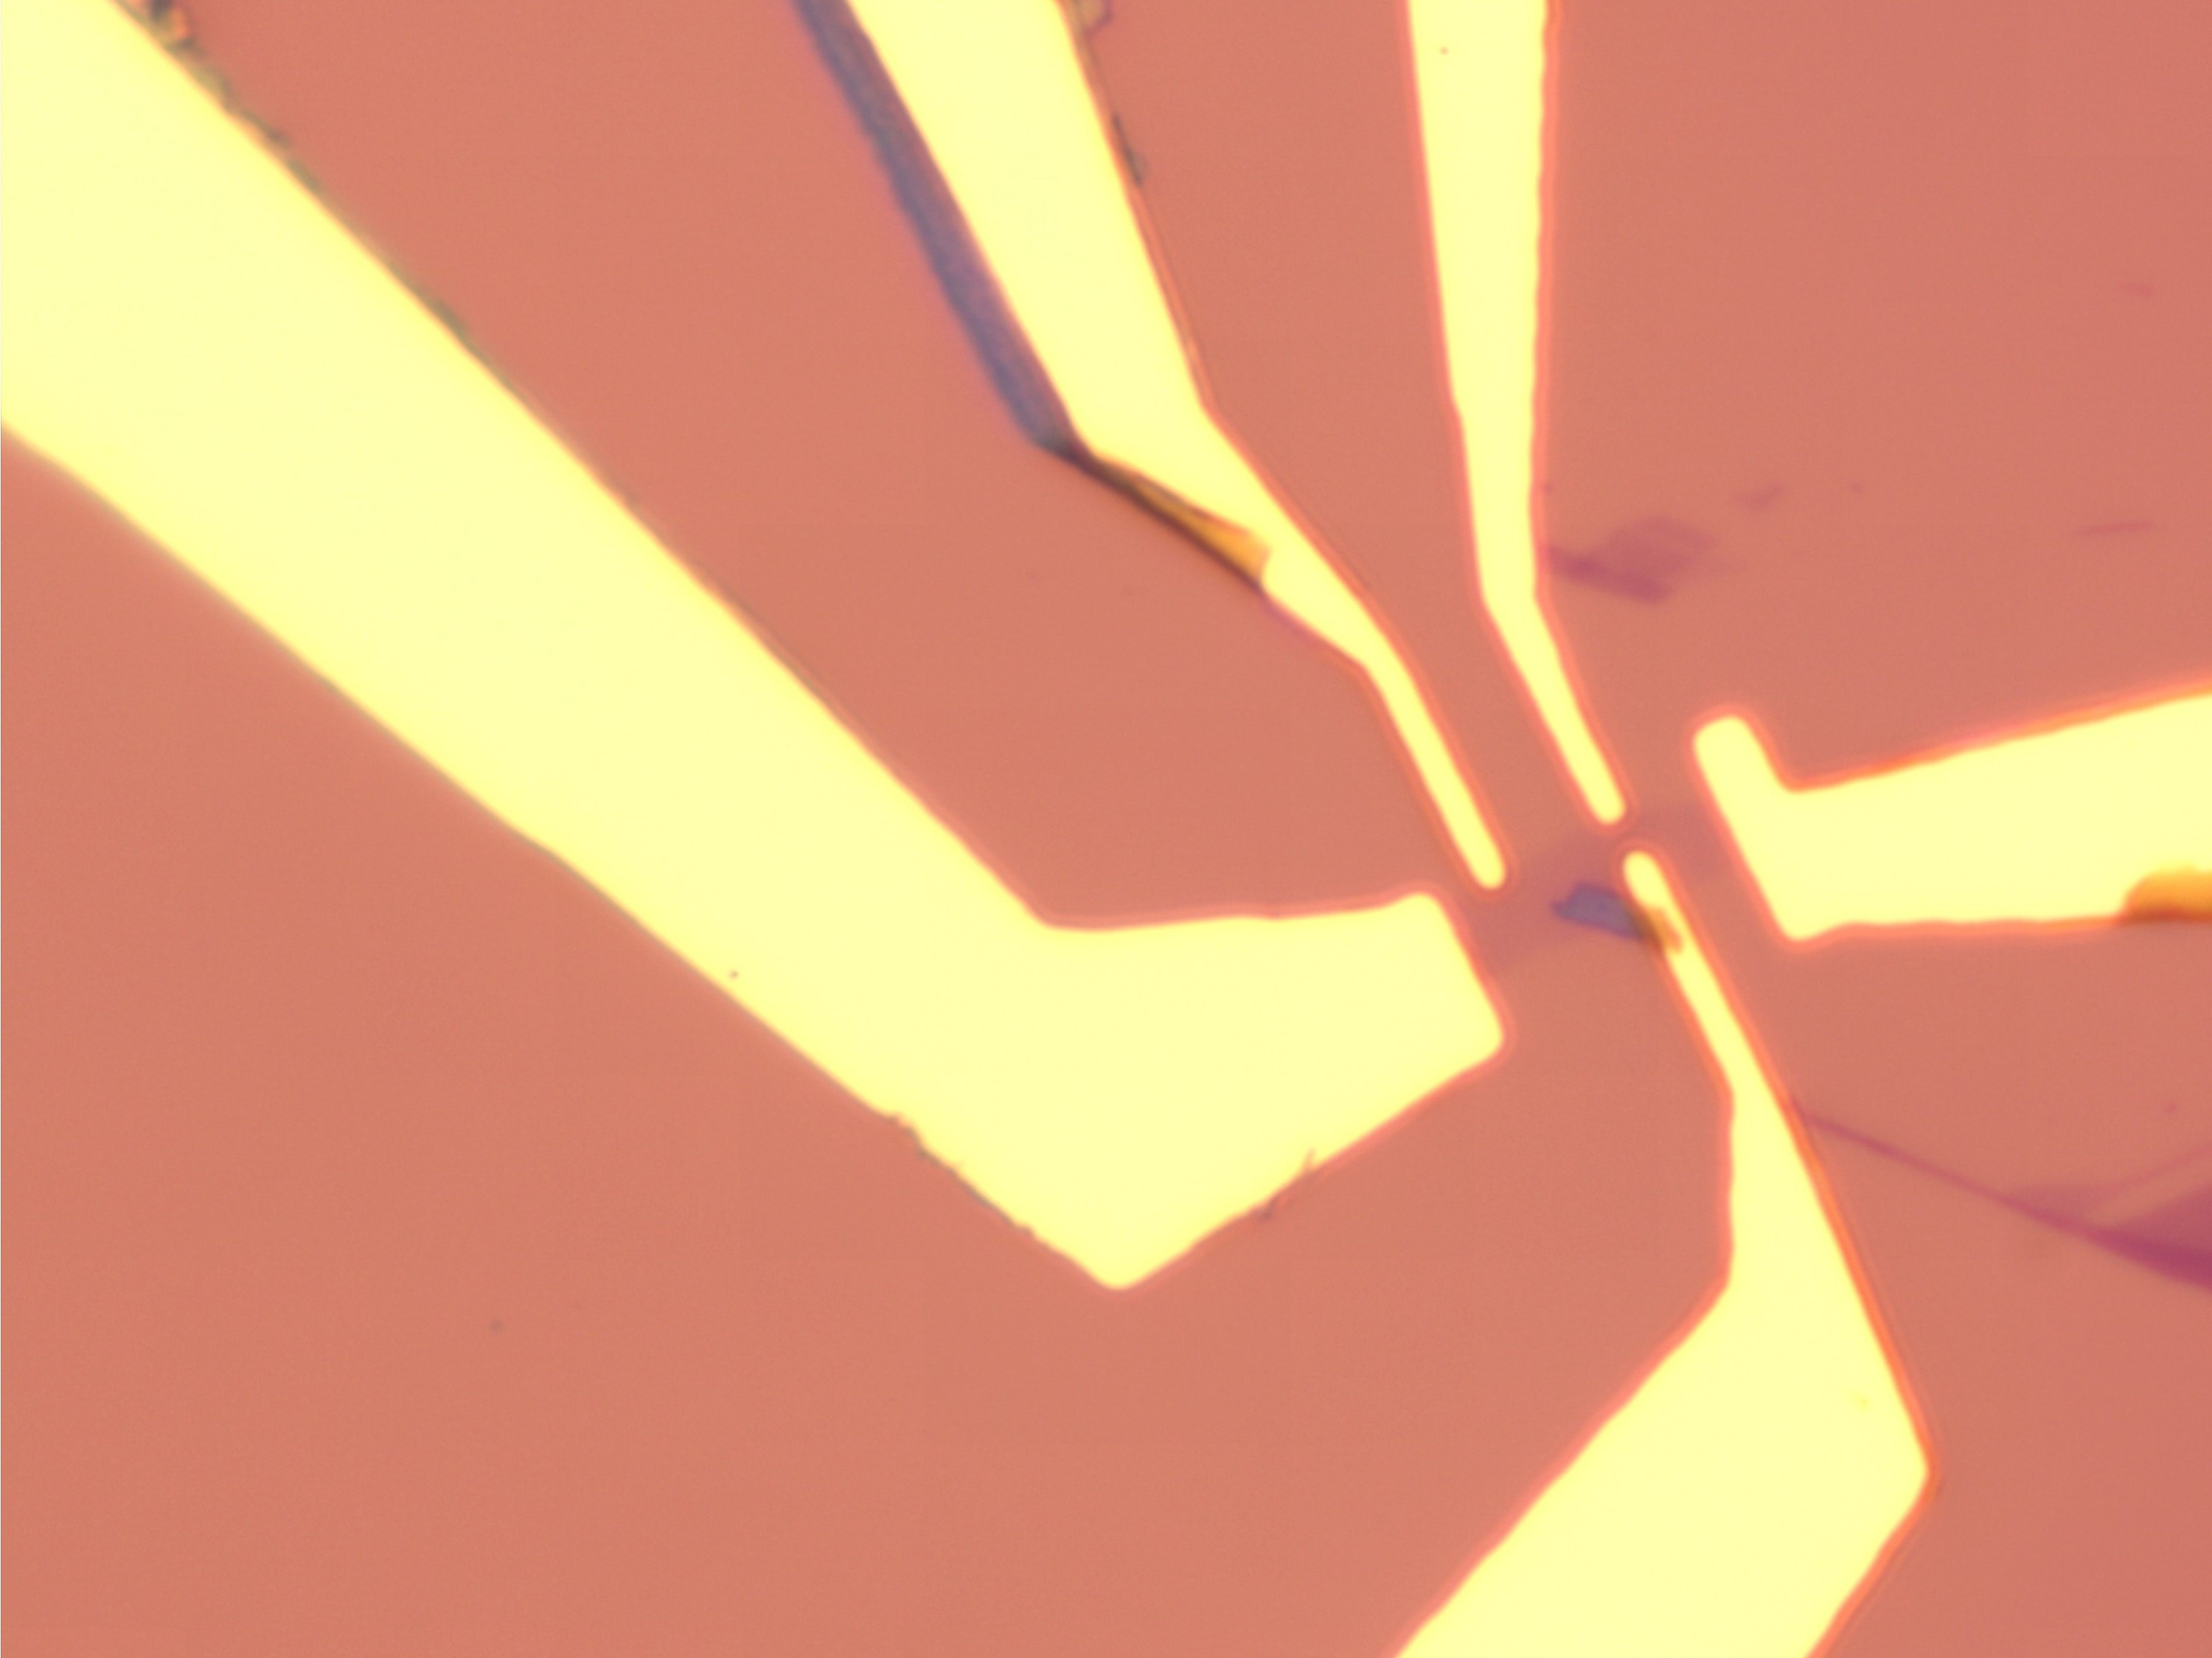
\includegraphics[width=\textwidth]{chap2/US/1_b}
			\caption{After 4s ultrasonication}
		\end{subfigure}
		\begin{subfigure}[b]{0.3\textwidth}
			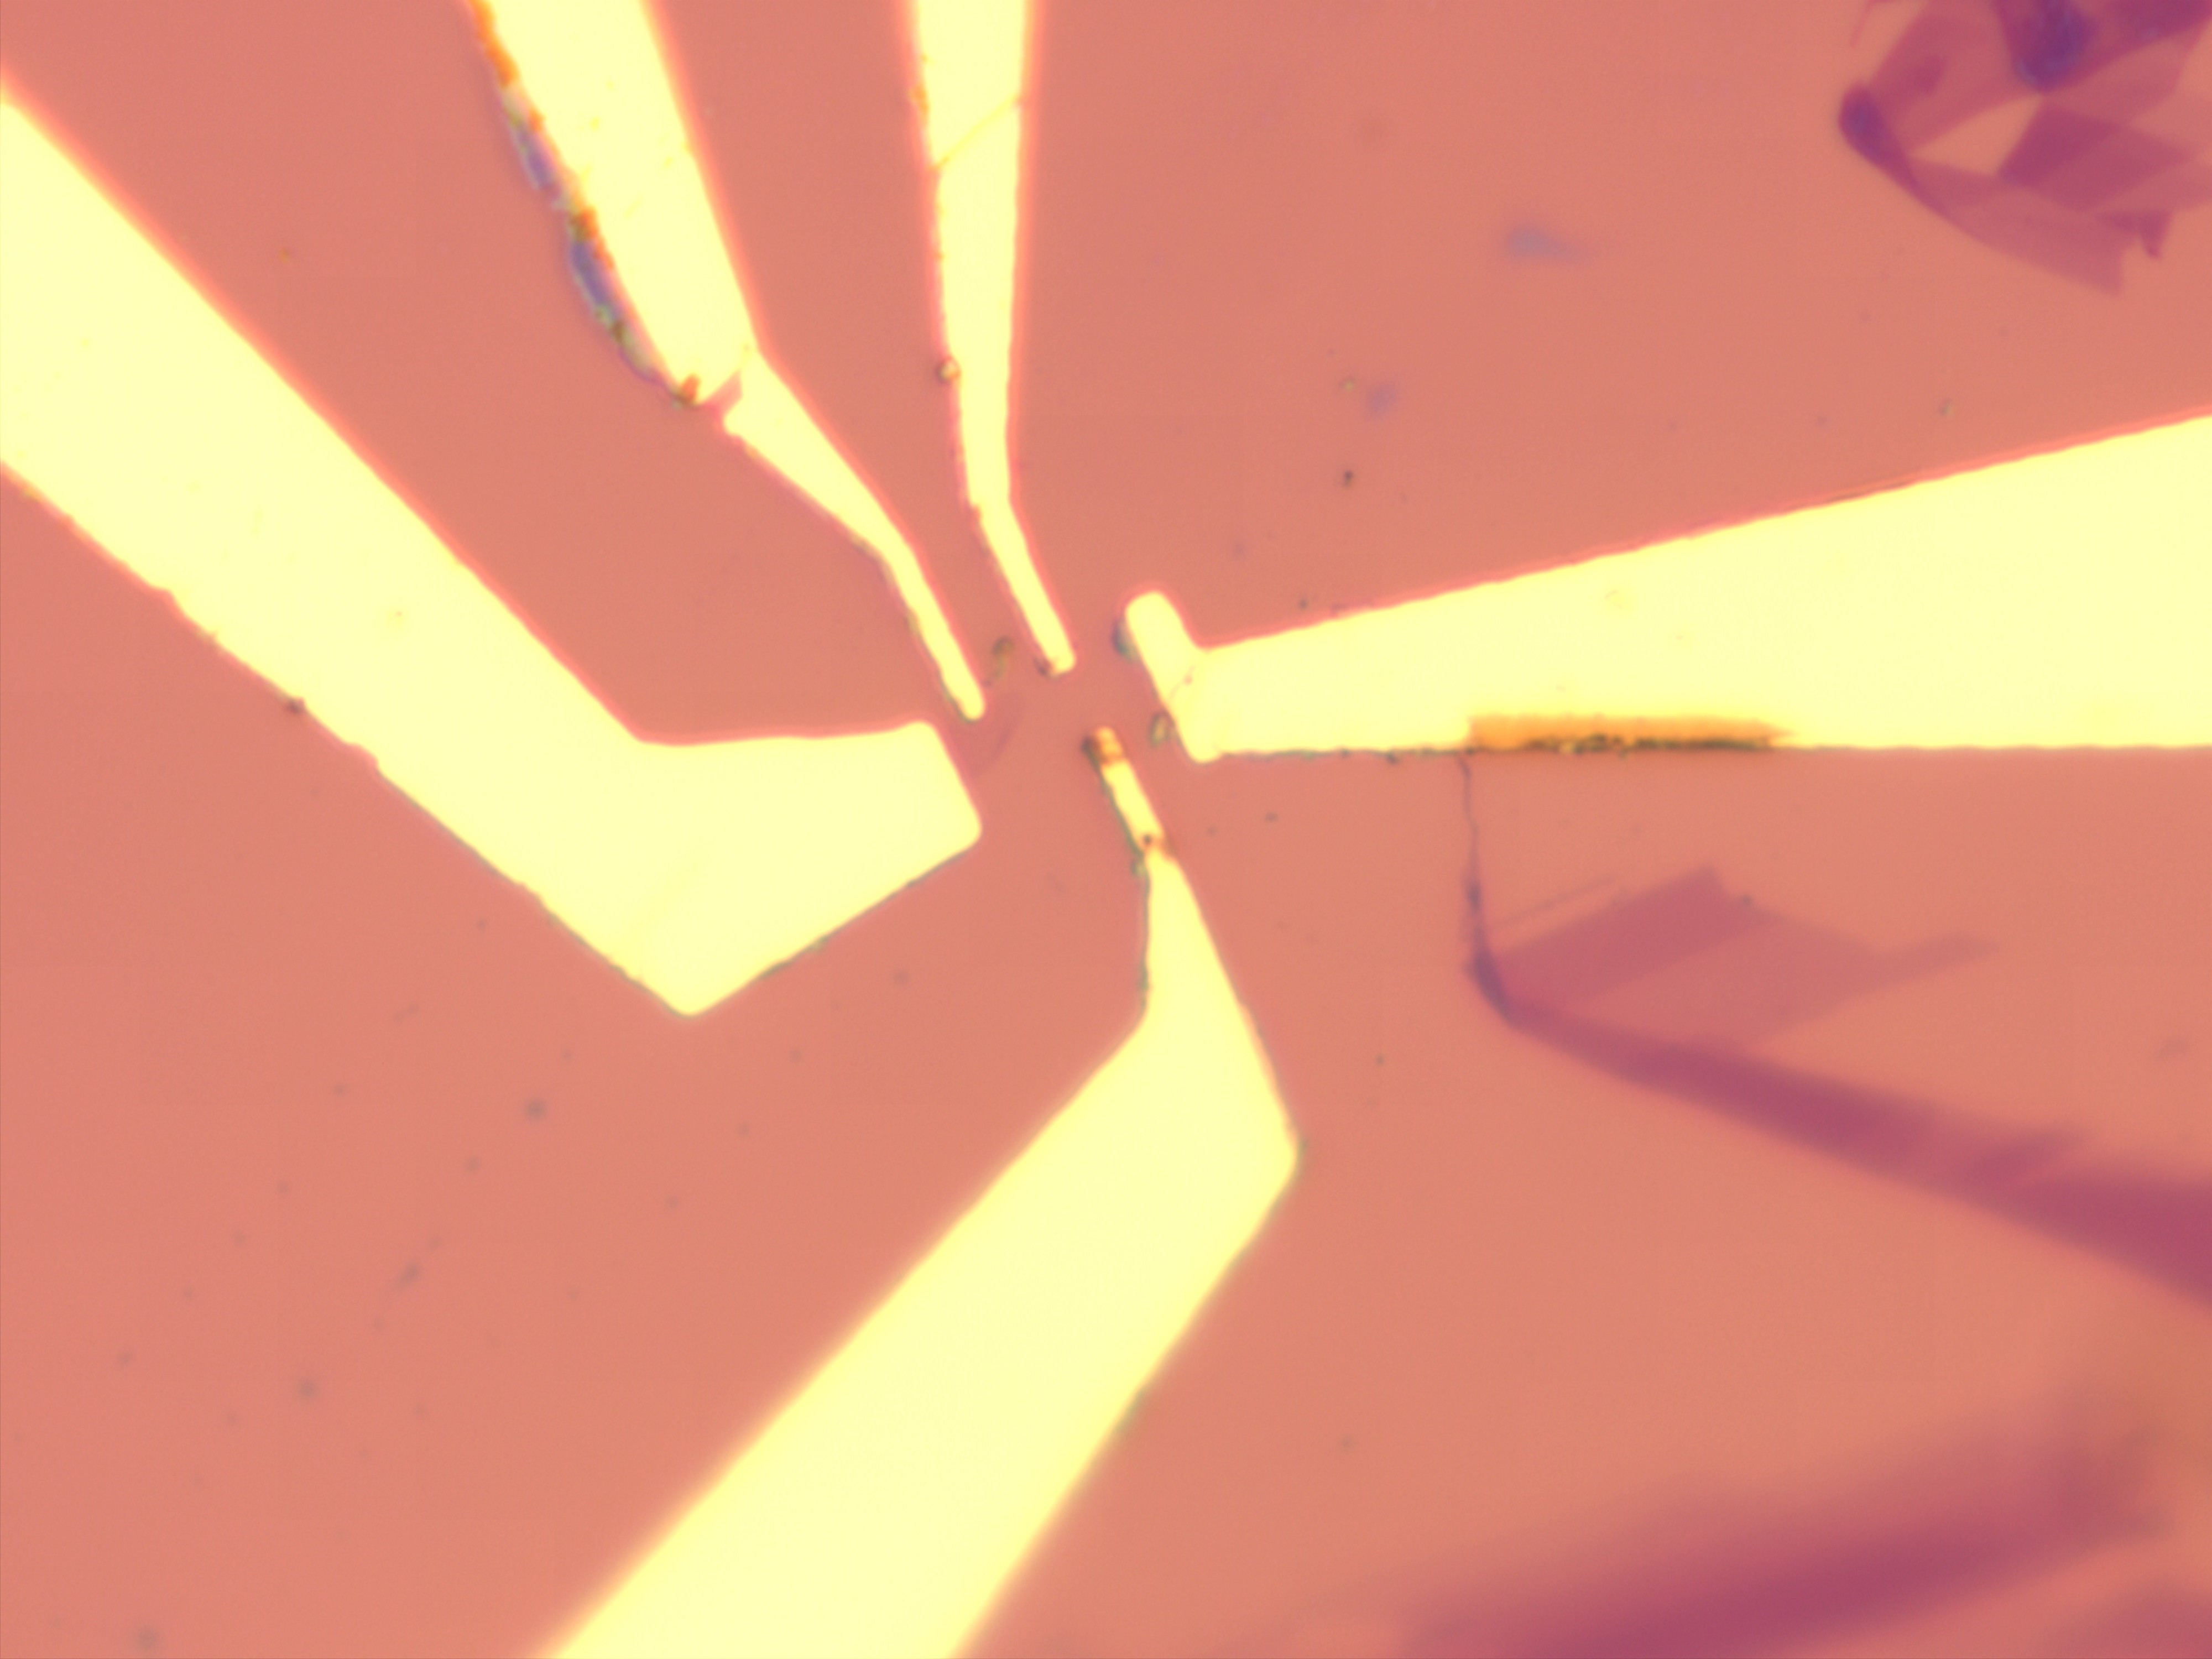
\includegraphics[width=\textwidth]{chap2/US/1_c}
			\caption{After 6s ultrasonication}
		\end{subfigure}
		\caption{Ultrasonication that has broken graphene sample.}\label{fig:lithography_skins_break}
	\end{figure}
	
	\paragraph{LOR-1A \& AZ-1512HS}
	An issue with a single layer photoresist processes is that well edges allow deposited materials to adhere, leaving 'skins'. One way to prevent this from happening is to use a multilayer process. Two resist layers are spun onto the sample, with the bottom film being more sensitive to the lithography process than the top (ie, develops faster, or is more sensitive to exposure). When developed, the bottom layer \textit{undercuts} the top layer, stopping adhesion to edges of the well when material is deposited. This process is depicted in \cref{fig:bilayer_lithography}.
	
	\begin{figure}[H]
		\centering
		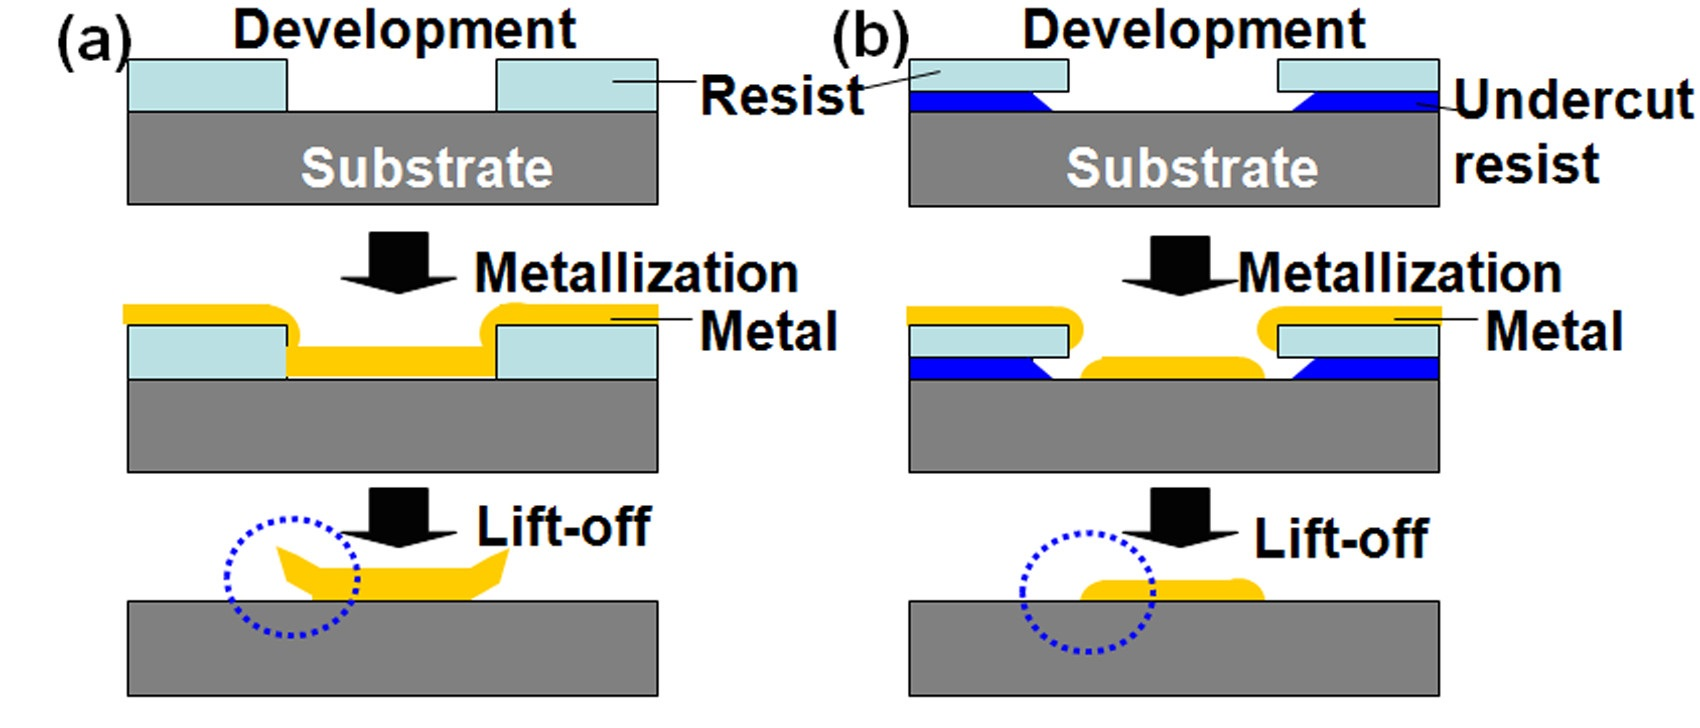
\includegraphics[width=0.5\textwidth]{chap2/bilayerResist.jpeg}
		\caption{Bilayer lithography process (Source: Park \etal\cite{park_bilayer_2008}) }\label{fig:bilayer_lithography}
	\end{figure}
	
	Rather than a photoresist, LOR-1A is a lift off resist. When the films are exposed to the developer, LOR-1A is also lifted off with the soluble AZ-1512HS. Additional material is pulled and dissolved from the well, leaving the desired undercut effect. %TODO CHECK HOW IT REALLY WORKS.
	
	\subsubsection{Exposure}\label{sec:exposure}
	After spinning, a mask writer tool is used to expose the wafer and resist films to UV light to develop desired pads. A mask writer usually is composed of a DMA (Digital Mirror Array) which allows filtering to pixel like squares. %TODO CHECK DMA
	
	An important parameter played with in this process is the exposure time, which affects your ability to develop fine structures. By using an array of different exposure times (\cref{fig:exposure_array}), we were able to optimise our feature exposure for a typical developing time.
	
	\begin{figure}[H]
		\centering
		
\includegraphics[width=0.3\textwidth]{placeholder}
		\caption{Developing an exposure array on \silicondioxide}\label{fig:exposure_array}
	\end{figure}
	
	Prepared CAD files, that specify the structure for desired contact pads onto devices, are used by the DMA to iteratevly expose small areas of the film. These exposed areas undergo a chemical change, changing the structural properties for development.
	
	\subsubsection{Developers}\label{sec:developer}
	Developers are used to dissolve exposed / unexposed areas of photoresist films. For example, we use AZ-726 in conjunction with AZ-1512HS. Using a development time complementary to your exposure time is important to not overdevelop your features, as material in prodximity to exposed areas is at risk of some structural damage. Developers do still affect the remaining structure over time.
	
	\subsection{UV Ozone surface preparation}\label{sec:uv_ozone}
	%TODO Cite papers here.
	Large resistances can occur when trying to make contact with graphene. This can be for a variety of reasons. Resist residues between the deposited pads and graphene can be insulating, non-metalic bonding between deposited metals and graphene, or oxidisation of metals being deposited (ie, chromium oxide).
	
	We use UV Ozone to clean the graphene exposed in our developed wells. UV Ozone cleaning blasts the surface with UV ozone light, while flowing oxygen gas. Overtime surfaces are slowly etched and material that is not strongly bonded is cleared. 
	
	In our optimisation we ran two wafers with devices at times of 5m and 15m respectively (see \cref{fig:UV_ozone}). The 15m devices were etched away completely, however the 5m device provided the first low resistance contact observed, after many iterations of devices.
	
	\begin{figure}[H]
		\centering
				
\includegraphics[width=0.3\textwidth]{placeholder}
		\caption{Cleaning before and after UV Ozone}\label{fig:UV_ozone}
	\end{figure}
	
	\subsection{Deposition}\label{sec:deposition}
	Once a designed structure is exposed to make contacts with graphene, 
	
	\subsubsection{Oxide Protection}\label{sec:deposition_oxide_protection}
	
	\subsection{Lift-off}\label{}
	\subsubsection{Ultrasonication}
	
	\subsection{Oxide transfer}
	% Introduction to metal stamping technique. Don't talk about optimisation here.
	
	
\end{document}